\documentclass{scrartcl}
% \documentstyle{article}
\usepackage{comment}
\usepackage{amsmath}
\usepackage{caption}
\usepackage{graphicx}
\usepackage{subfig}
\usepackage{wrapfig}
\begin{comment}

\end{comment}
\usepackage{xcolor}
\newcommand\todo[1]{\textit{\textcolor{red}{#1}}}

\DeclareCaptionType{mycapequ}[][List of equations]
\captionsetup[mycapequ]{labelformat=empty}

\providecommand{\comm}[1]{{\bf[ #1 ]}}
\providecommand{\commd}[1]{\comm{D: {#1}}}

\begin{document} 
%\title{Item Reponse Theory in Intelligent Tutoring Systems}
%\subtitle{Can IRT-based Learner Models used in an IRT Goals?}

%\author{Lieuwe Rekker}
%\maketitle


\begin{titlepage}
\begin{center}

% Upper part of the page. The '~' is needed because \\
% only works if a paragraph has started.
\newcommand{\HRule}{\rule{\linewidth}{0.5mm}}

\includegraphics[width=0.15\textwidth]{images/uva-logo.png}~\\[1cm]

\textsc{University of Amsterdam}\\[1.5cm]

\textsc{\Large Master's Thesis}\\[0.5cm]

% Title
\HRule  \\[0.4cm]
{ \huge \bfseries Item Reponse Theory in Intelligent Tutoring Systems \\[0.4cm] }

\HRule  \\[1.5cm]

% Author and supervisor
\noindent
\begin{minipage}{0.4\textwidth}
\begin{flushleft} \large
\emph{Author:}\\
Lieuwe \textsc{Rekker}
\end{flushleft}
\end{minipage}%
\begin{minipage}{0.4\textwidth}
\begin{flushright} \large
\emph{Supervisors:} \\
Dr.~Maarten \textsc{van Someren}\\
Diederik \textsc{Roijers} Msc.
\end{flushright}
\end{minipage}

\vfill

% Bottom of the page
{\large \today}

\end{center}
\end{titlepage}
\tableofcontents

\newpage

\nocite{labelcombi}
\nocite{lftransfer}
\nocite{importance}
\nocite{knowledgeproblem}
\nocite{modelreview}
\nocite{eirt}
\nocite{pfa}
\nocite{ktpfa}
\nocite{skillcombi}
\nocite{lfa}
\nocite{blackart}
\nocite{hambleton}
\nocite{newirt}
\nocite{bridge}
\nocite{ct}
\nocite{algebra}
\nocite{assessment}

%\listofmycapequs

\section{Introduction}

\subsection{Intelligent Tutor Systems}
An Intelligent Tutor System (ITS) is a computer program in which students answer question in order to learn. The questions are similar to pen and paper exercises that students would do from textbooks. However ITSs provide some advantages beyond simply being an electronic textbook. For one the ITS can provide direct and tailored feedback to the students answers and adapt the order in which exercises are presented based on their answers. 

Another advantage of ITSs is that they can easily record for every student what answers they gave to each question they were asked. This recorded data can be used to assess how well students know the material and can sometimes even be used to improve these ITSs and the questions they ask. A few of these datasets of student interaction with ITSs are available for research. The size and number of datasets available has let to the development of learner models.

\subsection{Learner Models}
Learner (or skill) models use the data of what student is asked what question as input and provide a probability of the answer being correct as output. One way to assess such a model is to take the last few questions answered by each student as a test-set, build a learner model on the remaining data and then see how well they predict the correctness of the answers on the test-set. This method corresponds to the standard method used in machine learning to evaluate models and is relatively easy, since accuracy of predictions can be calculated directly with the answers in the dataset.

For learner models it is preferred that they perform well at tasks such as assessing the level of a student or indicating the quality or difficulty of a question. Aside from the prediction accuracy, Desmarais and Baker (\cite{modelreview}) also mention using an external metric as the second option for evaluating models. Examples here would be the use of post tests or expert opinions. The disadvantage of these methods is that they are expensive and/or difficult to interpret. For example if new questions are added to an ITS or other changes are made it needs to be checked again if the model still performs well and thus the external measurements need to be repeated. Some of the learner models are based on item response theory where these problems have been worked on for a long time.

\subsection{Item Response Theory}
Item Response Theory (IRT) originates in the fields of psychology and more specifically psychometrics and was developed to standardize testing. Testing data are identical to the data from ITSs: students answer's to questions are recorded. The models used in IRT also work similarly to the learner models: the IRT models provides a prediction of whether a particular student will answer a particular question correctly. This is achieved through latent parameters that represent student skill, item difficulty etc. Since the goal is standardized testing, IRT is not interested in prediction accuracy, but in whether the parameter values for student skill, item difficulty etc. are approximately correct. To evaluate the performance of the model a group of experts could examine students and questions and determine the skill level of the student and the difficulty of the questions (thus using an external metric) and see if those match the parameters found by the model. This would be costly as each test would need an experts' judgment. Instead a variety of methods is used to see if assumptions of the models hold (for examples see \cite{hambleton} and \cite{newirt}). The most important of these is that the parameters that are found are invariant. This means that when similar tests would be given to a group of students, or if different students would take a similar test, the parameters of the students and the test items in the model would not change.

\subsection{Research Subject}
The resemblance between the data used in IRT and ITSs has made it easy to adapt IRT models to ITS data. A few of these models have been developed, but none of these use (adapted) methods use the parameters obtained directly or evaluate the model based on the parameters. In this research invariability of the parameter of these models is researched with ``To what extent are the knowledge component parameters invariant?" as its main question. The idea behind the question researched and the methods used is to explore the possibilities of using these learner models in ways similar to IRT models, without necessarily using external metrics.

\subsection{Overview}
In the models section an overview will be given of the IRT models, how their parameters are fit and how these models are evaluated. The models section also introduces the IRT based learner models.

In section \ref{sec:RW}, some background on the IRT based learner models is given and related research on the topic of evaluating parameter values of learner models instead of prediction accuracies is presented.

In the research question section the research question and some subquestion are formulated together with an outline the approach taken to answer them.

The methods section describes the experiments performed in detail, explains some of the metrics used and further underpins why the chosen approach is taken.

The results section presents the results of the experiments and offers an interpretation on the results. Additionally it describes extra steps taken outside of the initial approach to investigate some anomalies in the obtained results.

In the final section the conclusion on the subquestions and main research question is put together and discussed. Some remarks on possible improvements to the used methods and promising paths for future research are offered.

\section{Models}
In this section the subjects of this research are introduced: the IRT based learner models. First the data is described and the terms used to refer to its different parts are defined to make further discussion easier. Since the IRT based learner models are based on existing IRT models, the three basic IRT models and some background on IRT are described next. Finally the LFA, PFA and eIRT models are described by discussing how the IRT models are adapted to the ITS data.

\subsection{Data Form and Terminology}
The data for IRT models and the data for the IRT based learner models look the same. The data concerns a number of students (users of the system who answer `questions') and a number of items (the 'questions' asked). Characteristic for an item is that for each a single answer is expected. It might thus be that what normally is considered a single `question', is split up into multiple items. For example, ``What is the circumference and the area of a circle with diameter 2?" would be two items as two answers are expected. A question in the context of this thesis is one specific item asked to one specific student. This is the only meaning in which `question' will be used from this point on. Finally, an answer is here defined not as what answer was given exactly, but whether the answer was correct or incorrect. The data consists of questions and their associated answers, where every question-answer pair is a single data-point.  

\subsection{IRT Models}
At the basis of an IRT model are parameter-types that are either defined as student parameter-types or item parameter-types. For each student parameter-type a parameter is defined for every student and for each item parameter-type a parameter is defined for every item. Parameter-types stand for characteristics such as student ability and item difficulty. For each question the parameters of the student involved in the question and the parameters for the item involved in the question are combined with the logistic function (see formula \ref{eq:logistic}) to obtain the probability $P$ that the question is answered correctly. $\sigma(x)$ will be used throughout this thesis as it is the basis for both the IRT models and the IRT based learner models. Below the three basic IRT models are defined, after which the method of finding the parameter values and evaluating those values is discussed. 

\begin{comment}
As was mentioned in the introduction, an IRT model takes a question (i.e. the item asked and the student to whom it is asked) as input and returns the probability, $P$, that the question is answered correctly as output. The function at the basis of calculating this probability in each IRT model and all the IRT based learner models is the logistic function (see formula \ref{eq:logistic}). The different IRT models mostly differ in how $x$ is defined. Parameters of the item and student involved in the questions are combined in $x$. Generally only a single parameter for students is defined (student ability), while the number of parameters for items and how they are all combined into $x$ varies between the different IRT models.
\end{comment}
 
\begin{equation}
\label{eq:logistic}
P = \sigma(x) = \frac{1}{1+e^{-x}}
\end{equation}

\subsubsection{1PL or Rasch Model}
\label{sec:1PL}
The 1PL model, also known as the Rasch model has one student parameter-type ($\theta$) and one item parameter-type ($b$). The probability of a correct answer to a question follows from Formula \ref{eq:1pl}. $i$ and $s$ are the item asked and the student to whom the question is asked. $\theta_{s}$ represents the ability of the student $s$ and $b_{i}$ stands for the difficulty of the item $i$. It follows from this formula that when the skill of the student and the difficulty of the item are on a par, the student has a probability of .5 to answer the question correctly. 

\begin{equation}
\label{eq:1pl}
P(s,i) = \sigma(\theta_{s} - b_{i})
\end{equation}

For this model there is an indeterminacy issue. This means that different parameter values of a model can lead to exactly the same outcomes. In this case the issue lies in the fact that decreasing all $\theta$ and $b$ values by the same amount keeps the $P$ for any question constant. To be able to compare different sets of parameter values, this problem is generally solved by a transformation, such that the average $\theta$ becomes 0, while all $P$ of the model remain the same.

\subsubsection{2PL Model}
The 2PL model expands the 1PL model with the item parameter-type $a$ which is called the discrimination (see Formula \ref{eq:2pl}). The term discrimination comes from the fact that for an item with high discrimination, $P$ changes quickly with small changes in student ability when $|(\theta_{s} - b_{i})|$ is small and thus the performance of students who are close in skill can be more easily distinguished. The flip-side of a high discrimination is that when $|(\theta_{s} - b_{i})|$ is not small, $P$ will more quickly drop to 0 or rise to 1, concealing any difference between ability levels at those levels. 

\begin{equation}
\label{eq:2pl}
P(s,i) = \sigma(a_{i} (\theta_{s} - b_{i}))
\end{equation}

For this model indeterminacy is an issue: not only can all $\theta$ and $b$ be increased or decreased by the same amount, but all $a$ can be scaled up or down as long as all $\theta$ and $b$ are scaled down or up respectively by the same factor. For comparison of models a transformation is used so that the average $\theta$ becomes 0 and the standard deviation over all $\theta$ becomes 1, while all $P$ remain the same. 

\subsubsection{3PL Model}
The 3PL model adds the item parameter-type $c$ to the 2PL model. This parameter stands for the probability that on some questions a student who does not know the right answer, could still answer correctly by taking a guess. This phenomenon is most prevalent in multiple choice tests where the chances of correctly guessing the answer are high. The model effectively changes the lowest probability to the level of $c$ and the space between $c$ and $1$ is rescaled accordingly. The resulting Formula \ref{eq:3PL} is an adaptation of the logistic function.

\begin{equation}
\label{eq:3PL}
P(s,i)= c_{i} + \frac{1-c_{i}}{1+e^{-a_{i}(\theta_{s} - b_{i})}}
\end{equation}

The 3PL model suffers from the same indeterminacy issues as the 2PL model and is dealt with in the same way. This model completes the discussion of the three basic IRT models. The absence of multiple choice questions in the datasets used for this thesis removes the need for this model and thus it is not mentioned again. 

\subsubsection{Fitting the Models}
Before a model can be used to determine probabilities of correct answers for questions it is necessary to obtain values for all the parameters. Issue with these parameters is that none of them are directly observable (i.e. they are latent) and have to be obtained from observations indirectly. Instead the parameters are given those values at which the likelihood that the observed answers arise from the model is maximized. The likelihood of the answer to a single question is the probability that that answer is seen according to the model. Thus if the answer is correct, the likelihood for that answer is $P$, while if the question is answered incorrectly the likelihood is $1-P$. By taking the product of the likelihoods of each data point the likelihood of the entire dataset is determined, which results in formula \ref{eq:likely}. In this formula $D$ is the dataset, $d$ is a data-point and $t_{d}$ is the observed answer of data-point $d$ which has a value of either 0 (incorrect) or 1 (correct). $P_{d}$ is the probability according to the used model that the answer to data-point $d$ is correct.

\begin{equation}
\label{eq:likely}
L(D)=\prod_{d \in D} P_{d}^{t_d}  (1- P_{d})^{1-t_d}
\end{equation}

In the 1PL model the argument in $\sigma(x)$ is linear in the parameters, which makes it possible to use logistic regression. In the 2PL model $x$ is bi-linear and thus logistic regression can not be applied directly. Instead initial values for student parameters are randomly generated and kept fixed (making $x$ linear again) while logistic regression is applied. The found item parameter values are kept fixed as logistic regression is used to find the values for the student parameters. This procedure is repeated until the likelihood of the data is (nearly) the same in consecutive iterations. For more detailed information on logistic regression and how it is used here, please refer to appendix \ref{app:math}.

Note that this model cannot be used if a student answers all their questions correctly or incorrectly (the students ability will run to plus or minus infinitely respectively) or if an item is always answered correctly or incorrectly. To prevent this issue questions belonging to such students and items are removed from the data before fitting.

\subsubsection{Information Function}
\label{sec:inherent}
If an IRT model is considered to perfectly determine the observed data, there is still a random element in the data: when the probability of a correct answer is 90\% according to the model, an incorrect answer is still expected in 10\% of the cases. If the model would noiselessly generate the answer to the same set of questions twice, some differences between the dataset would exist. This means that even though the parameters used to generate this data and the questions asked are exactly the same, the parameters found in the fitting process would be different for each generated dataset. This variance in the found parameters cannot be prevented as it is part of the model and it is good to know how large this variance is, as it is a lower bound for the actual variance of parameters.  

In IRT information functions are defined which can be used to calculate the variance caused by the stochasticity. Baker \cite{basicbaker} describes an item information function as a function based on a set of items (with known parameters) that returns the variance in ability for a student that would be found if a student would answer this set of items over and over again, while every time forgetting he has seen these items and a model would be fitted to each set of results. 

The independent variable in this item information function is the ability of the student. The reason becomes clear from a small thought experiment. If a students ability is so low that he would probably give only wrong answers to the set of items, the estimates will be very inaccurate: the value of his ability could be a large negative value, but it might just as well be twice as big. Students with about average ability probably give a correct answer to about half the items, leaving far less uncertainty about their skill.

In IRT the item information function is most important as it is used to choose items with known parameters for an exam, such that the variance for every expected ability level is low. An equivalent information function can also be made though for a group of students (again with known parameters) where, given parameters for an item, the variances for that item's parameters is given. This is important when considering how many students are needed to accurately obtain parameters for a new item to be included in tests. 

%In both these  only the the set of questions is of importance for the information function while the answers are irrelevant. The answers do influence the found variances indirectly through their influence on the fitted value of the parameters on which the information function is dependent.

%The idea of the information function is adapted to the learner models later in this thesis. As none of the parameters are known the  

\subsubsection{Assessment of Parameter Values}
\label{sec:asses}
Measurements of how well the model makes predictions can be obtained directly by looking at its predictions on a testset and comparing these to the actual answers. The objects of interest in IRT, the parameter values used to make these predictions cannot be directly observed, which poses a challenge in assessing the obtained parameter values. Through the use of experts it is possible to get an indication of what parameter values are correct, but this would at least be costly and still poses additional problems (e.g. even experts amongst each others can disagree). There is thus no easy direct way to check the validity of values of the parameters. In \cite{hambleton} Hambleton recommends using three types of indirect evidence to evaluate the parameters values of a fitted model:

\begin{quote}``[J]udgements about the fit of the model to the test data [should] be based on three types of evidence: 1. Validity of the assumptions of the model for the test data 2. Extend to which the expected properties of the model (e.g., invariance of item and ability parameters) are obtained 3. Accuracy of model predictions using real and, if appropriate, simulated test data."[p.55]
\end{quote}

The most important assumption meant in the first type of evidence is that of unidimensionality: the ability represented by $\theta$ should be the only ability of importance in answering the items. A good example of when this assumption is broken, is when an item on a math exam uses difficult wording for an easy math problem, making both the students' ability in math and their close reading ability important in answering this item correctly.  

The second type of evidence and especially the mentioned example of invariance, is of major importance for IRT. In Hambleton's own words: ``The property of invariance of item and ability parameters is the cornerstone of IRT". Invariance means that the parameters obtained for items and students have low variance. Partly this variance is already expected through the information function and generally the amount and choice of data (i.e. what items or what students are used in a test) is adapted to this. There might also be other sources of variance in the parameters. One of these reasons is that assumptions of the model are broken. An example put forward by Hambleton to inspect invariability is to split the students/items in two and see if the parameters of the items/students fit on the two different sets (taking the indeterminacy issue into account) resemble each other. The method he uses for this is to plot them against each other and see if this plot produces a straight line. He states that the property of invariance should be checked even more stringently, and one of the methods he uses is to split the students/items in such a way that the highest skilled/most difficult ones are in one group while the lowest skilled/least difficult ones are in the other and repeat the same procedure. He concedes that some more scatter is expected at the low and high ends of the parameter scales due to the higher inherent variance discussed in the previous section. 

The advantage from this method can be seen from the example given for the previous type of evidence: if we assume that language skill is independent of math skill, question that strongly depend on language skill will receive a higher difficulty parameter on the high ability dataset compared to the lower ability dataset. A variant of this method will be used to look at the invariability of parameters found in our learner model. The specifics of how this is done are described later. 

His third point refers to metrics of model fit and model prediction. These are easy to obtain and if the predictions by the model for questions that were not used in fitting are inaccurate, the model is probably not a good fit for the data. An advantage of this type of evidence is that it can easily be obtained. These kind of measures of fit of the model will also be used in this paper and are described in detail later as well. 

\subsection{IRT based learner models}
Although the models used in this research are based on the 1PL and 2PL models, there are also three important differences. The first and most obvious is that they incorporate learning, as students' ability levels are expected to increase as they answer questions in an ITS, since the ITS facilitates the learning of students through feedback. To represent this, ability in the model, $\theta$, is split up in an initial part and a learned part, such that each time they answer a question the students ability increases.

The second major difference stems from the difference between the data used for the IRT models above and the ITS datasets used for the learner models. As said before the data for IRT models and the data from the ITSs used in this thesis look the same, but in the ITS data there are multiple different abilities and moreover a single item can involve multiple abilities. The name for one such ability in these datasets is knowledge component (KC). The ITS datasets thus do not only contain datapoints, but also a mapping of what KCs each item is associated with.
This change also means that the learner models are no longer unidimensional. The unidimensionality assumption is replaced with the assumption that any ability that influences the answer to an item is contained in the mapping of items to KCs.

Finally a subtle but major change was made to the item parameters in the model. Instead of defining parameter per items, parameters are defined per KCs. Thus in these models an item is associated with one or more Knowledge components that have their own difficulty level etc. Items now have their influence on $P$ through the parameters of the KCs they are associated with. From a data perspective this makes sense as the number of knowledge components is smaller than the number of items (here ranging from 8 to 1000 times as small, depending on the dataset), this greatly reduces the number of parameters that need to be fit. 

\subsubsection{Learning Factor Analysis (LFA)}
\label{sec:AFM}
The LFA model (or alternatively additive factor model: AFM) has the 1PL model as its basis, but extends it by introducing a learning rate as discussed in the introduction and by allowing multiple knowledge components to be associated with a single item. The combination of KCs is made by summing the learned part of knowledge and the difficulty of the KC for every KC that is linked to the item.

\begin{equation}
\label{eq:afm}
P(s,i) = \sigma(\theta_{s,0} + \sum_{c \in KC_{i}}(\gamma_{c} t_{s,c} - \beta_{c}))
\end{equation}

In the LFA model (see Formula \ref{eq:afm}) student ability is split into an initial ability parameter, $\theta_{0}$, (defined per student) and a learning rate, $\gamma$, defined per KC (i.e. the KC determines how fast or slow learning occurs) which is  multiplied by the number of times that a student has seen items associated with this particular knowledge component, $t_{s,c}$. Learning is thus modeled by increasing a student's ability for a KC by a fixed amount each time they encounter an item involving that KC. The involvement of multiple KCs is implemented by summing over all KCs that are associated with an item $i$. For each of these KCs, the students' learned part minus the difficulty part for each KC (indicated by the subscript $c$) is added.  

In the the original LFA model $\beta$ is added, instead of subtracted. It is subtracted here to maintain similarity to the original IRT models and ensure uniformity with the other models used. This has no other effect than that the signs for $\beta$ are reversed.

The indeterminacy that can occur in the 1PL model (discussed in section \ref{sec:1PL}) is absent here when items are associated with a different number of knowledge components (which is expected as the number of KCs associated with items differs between items within every dataset used). When raising $\beta$ and $\theta_{0}$ by the same amount (the indeterminacy in the 1PL model), items with more associated KCs are affected more by this increase through the sum, changing the Ps, thus no longer leading to the same model. 

\subsubsection{Performance Factor Analysis (PFA)}
\label{sec:pfa}
The PFA model is a direct extension of the LFA model. In the PFA model separate learning rates are used for questions answered correctly and questions answered incorrectly. Additionally $\theta_{0}$ is dropped, which as put forward in \cite{pfa}, was done to improve the predictions the model can make: not having any student specific parameters makes the model applicable to students not used in the fitting procedure for whom no $\theta_{0}$ value would be available. As noted in both \cite{ktpfa} and \cite{blackart}, leaving out $\theta_{s,0}$ makes parameter estimates worse. Since we are only concerned with students for whom data is included in the data-set, a model that does include $\theta_{s,0}$ (as done in \cite{ktpfa} and \cite{blackart}) is used instead of PFA and will be referred to as PFA+.

\begin{equation}
\label{eq:pfa}
P(s,i) = \sigma(\theta_{s,0} + \sum_{c \in KC_{i}}  \gamma_{c} g_{s,c} + \rho_{c} f_{s,c} - \beta_{c})
\end{equation}


Here $\gamma$ is the learning rate of the KC for correct answers and $g_{s,c}$ is the number of questions concerning KC $c$, answered correctly by student $s$. $\rho$ is the learning rate of the KC for incorrect answers and $f_{s,c}$ is the number of questions answered incorrectly. The idea behind this model thus is that students make a different gain in ability when answering a question correctly than when they answer a question incorrectly. Just as with the LFA model above the sign for $\beta$ is reversed compared to the original representation of the model.

\subsubsection{extended Item Response Theory (eIRT)}
\label{sec:eIRT}
The extended Item Response Theory model by Roijers et al \cite{eirt} is an extension of the 2PL model. It is different from the previous two models in that it is unidimensional: i.e. each item is only associated with a single KC (called rule in \cite{eirt}) (Note that although only a single KC is associated with each item, there are still multiple KCs overall). The eIRT model still splits $\theta$ into an initial skill and a learned part. 

\begin{equation}
\label{eq:eIRT}
P(s,i) = \sigma(\alpha_{c} (\theta_{s,0} + \eta_{s} t_{s,c} - \beta_{c}))
\end{equation}

Although the incorporation of a learning rate is similar to the above two models, there is a major difference: here the learning rate is a student parameter-type rather than a KC parameter-type. Also, with $\theta$ split up, it would seem that $\alpha$ obtains a slightly different meaning. For $\theta_{0}$ it still has the same discriminatory function. When looking at $\eta$ though, $\alpha$ directly impacts it as a modifier, making learning easier ($\alpha>1$) or more difficult ($\alpha<1$) for that knowledge component.

As this is a unidimensional item the problem of indeterminacy is also present here exactly as it was in the 2PL model. Comparing parameter values can be can be done in the same way as in the 2PL model.

\subsubsection{Multidimensional eIRT}
As described above, eIRT does not incorporate multiple skills (KCs) per item. In order to be fitted on the multidimensional data used in this thesis, we introduce a multidimensional version of eIRT here. This multidimensional eIRT (meIRT) is made to deal with the multidimensionality of the data in the same way as LFA and PFA+, resulting in formula \ref{eq:sumeIRT}. $\theta_{s,0}$ is now included in the sum because it should be affected by $\alpha_{c}$ as it is in eIRT while it is also divided by the number of KC's that is summed over to ensure $\theta_{s,0}$ is on average added once, as it is in LFA and PFA+.


\begin{equation}
\label{eq:sumeIRT}
P = \sigma(\sum_{c \in KC_{i}} \alpha_{c}(\frac{\theta_{s,0}}{|KC_{i}|} + \eta_{s} t_{s,c}) - \beta_{c})
\end{equation}

Please note that in the multidimensional case the indeterminacy where all $\theta$ and $\beta$ can both be shifted by the same amount is in normal circumstances no longer there as was described for the LFA model. The indeterminacy concerning $\alpha$ and the student parameter-types still exists though and is resolved by making the standard deviation of $\theta_{s,0}$ equal to 1 and changing the other parameters accordingly. 

\begin{comment}
\subsubsection{Combining knowledge components}
\label{sec:comb}
Something more can be said about the way KCs are combined. In \cite{skillcombi} Cen et al. show that in practice there is no difference in performance between an additive model (as used here) or a conjunctive model (where probabilities of individual KCs are multiplied). Nevertheless the authors already mention that this is probably the case because for most KCs $\beta < \eta_{c} t_{s,c}$, meaning that adding KCs does decrease the chance of answering the question correctly as would be expected. In their paper they already propose using a data set where ($\beta > \eta_{c} t_{s,c}$) to see if this is indeed why this way of combining KCs works well in practice.

The experiment proposed above is put to the test here. Fitting a conjunctive model is hard in practice, but generating data using one is rather straightforward. Whether a real life data set contains many questions where skills are such that $\beta < \eta_{c} t_{s,c}$ cannot be said at this point. Even if this is not the case though, it can be argued that the parameter values can be skewed slightly to ensure that this occurs. The rationale behind is, is that the fitted values obtained from the real data may be skewed towards $\beta < \eta_{c} t_{s,c}$ due to a additive model being used in the fitting process. It would then be expected though that the retrieved parameters using these values would be skewed towards $\beta < \eta_{c} t_{s,c}$ again.

In comparing meIRT's (or eIRT's) parameter values to those of LFA $\beta$ should be multiplied by $\alpha$. $\theta$ is to be multiplied by a weighted average of $\alpha$ (according to the ratio of KCs of the questions that the corresponding student has answered). Finally a weighted average of $\eta$ per KC should be taken according to the ratio of questions each student has answered containing that KC. meIRT can be compared to PFA by combining the steps above with the steps needed to compare PFA to LFA.

\end{comment}

\begin{comment}
\subsubsection{Combined Model}
The three models introduced above can all be encompassed by a more complex model.

\begin{equation}
P = \sigma(\sum_{c \in KC}\frac{\alpha_c \theta_{s,0}}{|KC|}+\eta_{s} \gamma_{c} g_{s,c} + \eta_{s}\rho_{c} f_{s,c} - \beta_{c})
\end{equation}

LFA can be obtained from this model by taking $\alpha=1$, $\eta=1$ and $\gamma=\rho$. PFA can be obtained from this model by taking $\alpha=1$, $\eta=1$ and $\theta_{0}=0$ (minus the last one for PFA+). The adapted eIRF can be obtained by taking $\gamma=\rho=\alpha$ and realizing that $\beta$ already incorporates $\alpha$. It suffers from the same indeterminacy problem as the meIRT model, which can be dealt with in the same way.

\subsubsection{Model issue}
\todo{Somehow it seems to me that it is a major issue that these models are inconsistent: Students have only a single initial skill, while after learning skills diverge. This is rather odd as forgetting this past and fitting the model again would result in all these different levels being dumped into a single skill again.}
\end{comment}

\section{Related work and Background}
\label{sec:RW}
In this section first some background is given on where the LFA and PFA models come from. Then some of the research is described where parameter values are investigated, rather then simply looking at the predictive accuracy of the model. 
\subsection{LFA and PFA Model Backgrounds}
Learning factor analysis (LFA) is a method of analysis put forward in \cite{lfa} to obtain the best possible mapping of items to KCs. Each such mapping is called a cognitive model. The evaluation of a cognitive model is determined through the BIC and AIC values when fitting a LFA model on the data using that cognitive model. Both BIC and AIC incorporate the likelihood of the data given the model and penalize this relative to the number of parameters used in the model. The cognitive models considered in this paper are models proposed by experts and combinations of those models. This way they for example can tell if a particular KC should be split in two, or if two KC's should be merged into one. The authors inspect the implications for education of the resulting best models and conclude that this method has indeed produced better cognitive models with practical applications for education. 

The cognitive model in \cite{lfa} is generally called a Q-matrix. Others such as \cite{matrixfact}, \cite{qm1} and \cite{qm2} have looked at automatically generating Q-matrices from data as well, but will not be discussed here as the cognitive models provided with the datasets is used and no attempt is made to improve on them.

As knowledge tracing (KT) is often compared to the models used in this thesis a short explantion of it is given here. For a more extensive explanation please refer to \cite{kt}. Knowledge tracing works from the idea that students either know a skill or they do not. When students know a skill they still have a chance to incorrectly answer a question concerning that skill (this is called the slip parameter) and when students do not know a skill there is still a chance that they answer it correctly (the guess parameter). When students do not have a skill there is a chance of learning it after answering an item concerning that skill (the learning parameter). Once students have a skill, they cannot lose it. Finally when a student has not answered any questions concerning a skill yet, there is a base probability that a student knows this skill (the initial knowledge parameter). Note that all these parameters are defined per skill, so no student specific parameter is used. The parameters for this model are fitted as such that the likelihood of the observed data is maximized. The effect is the same as for the models used here, except that the procedure of finding the best parameters is more complicated (one method is resorting to brute-force searching). Given the parameters and answer of a particular student the probability that the student knows a skill can be calculated through iterative application of bayes rule on the answers. From there a prediction for the students next answer can be made. There is one important difference between the models: KT is made to apply to unidimensional data only (i.e. exactly one skill per item). In comparing the models this has led to splitting the observations for items with multiple kc's into multiple observations and various methods of obtaining predictions from the models. This makes the comparison of PFA and KT difficult.

The performance factor analysis (PFA) model is a further extension to the LFA model. It is introduced in \cite{pfa} as an alternative to knowledge tracing and focuses more on prediction accuracy, especially for making predictions for students not included in the fitted data. For this reason (as mentioned in \ref{sec:pfa}) PFA does not use a parameter for initial knowledge. In comparison with KT this makes sense as KT does not have any student specific parameters and thus a fitted model can readily be applied to students that were absent from the original dataset. By dropping the only student parameter, PFA gains the same advantage. The conclusion of \cite{pfa} is that the PFA model provides better predictions on a testset and is thus preferred over KT.

\subsection{Inspection of Parameters}
In \cite{ktpfa} Gong et al. also made a comparison between various knowledge tracing approaches (mostly differing in the fitting process) and PFA. Whether PFA or KT performs better remained inconclusive. Upon inspecting parameter values they found that many learning rates in the PFA model were negative, which seemed implausible in real life: unlearning from making exercises, because one gives the wrong answer, defeats the purpose of making exercises and would lead to a negative spiral. They noted that upon placing a lower bound of 0 on the learning rate, prediction accuracy improved. The authors do move beyond this focus on how well the models predict by looking at how well the initial knowledge parameter correlate to a pre-test made by the student. In this set-up the PFA+ model (which is described in section \ref{sec:pfa}) was compared to an adapted KT model that includes a starting knowledge parameter per student. In this setup the PFA+ showed a significantly higher correlation with the pre-test at 0.895. This indicates that the PFA+ model performs well at finding correct values for students' initial skill.

In \cite{knowledgeproblem} Beck also goes beyond investigating the accuracy of predictions of a model (knowledge tracing in this case) and looks at the parameter values. The authors prime reason for concern lies in identifiability: the fact that widely differing parameter settings can lead to almost identical model outcomes. Note that this problem is equivalent to the indeterminacy problem of IRT, but of more concern: in IRT the ordering of parameters is the same over all models with equal outcomes, while in the case of KT one KC could for example have a high guess parameter in one model and a low guess parameter in another models while the models still produce virtually the same probabilities for each data-point. 

Although Beck (\cite{knowledgeproblem}) does concern himself with the `plausibility' of parameter values he only goes so far as to nudge the parameter to values deemed plausible rather than asking whether the parameter values found are stable and accurate enough to be plausible, which is central to this thesis.

Yudelson et al. show some particular factors that can negatively influence the quality of PFA models. One of the factors looked at here is model complexity: on the one hand this is done by using a more fine grained set of KCs (i.e. a Q-matrix with more KCs) and on the other hand by adding a (uninformative) parameter to the PFA model. In evaluating their results the authors did not only look at prediction accuracy, but also inspected values for specific parameters and used an information-function equivalent to estimate standard deviations (deduced from personal correspondence with the author) In inspecting learning parameters they also noted how the learning parameter for wrongly answered questions are often negative when initial knowledge is not included in the model. They concluded that PFA not so much models student learning in this case, but rather performs some kind of `error tracking' in order to produce good estimates of skill. In other words, rather than modeling learning, it uses the mixture of right and wrong answers to estimate student skill: wrong answers indicate that a student does not have a skill and thus have a negative impact and vice versa for correct answers. Because of this the authors prefer an adaptation of PFA that includes initial student knowledge which is equal to the PFA+ model used in this thesis.

Roijers et al. focus mainly on the invariability and correctness of the parameter values in \cite{eirt}. They introduce the eIRT model described in section \ref{sec:eIRT}, alongside some variations where the initial knowledge and/or the learning parameter is not just dependent on the student, but also on the rule (corresponding to our use of KC) that is applied. These models were used to generate datasets using random parameters. Parameters of models fitted on this data were then inspected to gain an estimate of the invariability of the parameters. Here the conclusion was that invariability can quickly become a problem with these models (especially for the discrimination and learning parameters) and for the rest of their research the eIRT model is settled on.

In the second part of their research Roijers at al. used a dataset obtained from 14 students (from three different groups of students), using 23 rules and on average 6.1 answers per rule per student. This dataset was so small that the authors concluded from simulated data that the learning rate and discrimination parameters would not be accurate. To investigate if the initial knowledge parameter values were correct, they formulated a hypothesis on the ordering of average initial knowledge values per group, based on their perceived level of each group. 
The ordering of rule difficulty values was investigated by comparing them to orderings made by content experts. The hypothesis turned out to be correct and the obtained ordering of parameters was indistinguishable from those made by the content experts. Although this does not prove that these parameters are entirely correct it does indicate that they at least to some degree correspond to reality.

\begin{comment}
The method of using simulated data in estimating parameter variance was used in \cite{eirt}. Roijers et al. proposed a few alternatives to extending to the 2PL model, but after evaluating the variance of parameters on generated data settled on the extended IRT model described in section \ref{sec:eIRT}. At first they show that parameters can be retrieved from generated data. Additionally they also collected a data-set based on 14 students from three different groups. With the small amount of data in their collected data set, they concluded based on their previous experiment that only rule difficulty and student initial knowledge could be determined with enough accuracy, while learning rates could not. After fitting the model on the observed data the fitted initial knowledge of the three different groups confirmed their hypothesis of the ordering of average initial knowledge per group. Also the ordering of difficulty of the rules involved was found to be indistinguishable from rankings made by experts. The authors thus showed that the ordering of the difficulty and initial knowledge parameters obtained reflect the ordering of those in reality.
\end{comment}

\section{Research Question}
\label{sec:RQ}
Hambleton's statement that invariance of parameter values is `the cornerstone of IRT' is taken as the basis for this thesis. The main question investigated is ``To what extent are the knowledge component parameters of IRT based learner models invariant?" This question is broad and not clearly defined. In this section the main research approach and some subquestions are formulated to provide more clarity about what is looked into and why this is important. The methods described in this section only form an outline, which is further expanded upon in the next section.


\subsection{Research Approach}
The approach we use is inspired on Hambleton's prescribed method of splitting the data in two and plotting the fitted values of the parameters against each other. A more quantifiable approach is taken by splitting the data in more than two parts to see how invariant parameters are over these parts.

Splitting the data into parts poses some issues as to how the data should be split. In this research the parts are made by splitting the data in sets of students. The details and reasons of this method are explained in the next section, but the effect for the research question is that only the parameters that are defined per KC will be looked at.

\subsection{Subquestion: Parameter Variance}
The first subquestion directly looks at the variance of the parameters over the models fitted on the different parts. This is of importance when for example estimating how long a student needs to work on a particular KC to gain a firm understanding. This subquestion is formulated as: ''What is the standard deviation of the KC parameter values over subsets of the data?"

\subsection{Subquestion: Parameter-type Ordering Invariance}
In the research of Roijers et al., discussed in section \ref{sec:RW}, the authors did not look at the variance of parameters when researching the model fitted on real data, but rather looked at if the orderings of the parameter values within a parameter type were different. Thus not the variance per parameter is looked at, but rather the ordering of values within a parameter type is checked: i.e. is each parameter still in the same position when ordering on the magnitude of the values. This method is used here as well. So not only the invariance of the parameters is investigated, but also the invariance of the parameter ordering within each parameter-type. This is done because, just like in the case of Roijers et al. the interest is not always in the values of the parameters, but sometimes in whether or not the ordering of the parameters is correct: i.e. it is not investigated how much more difficult one KC is compared to another, but which one is more difficult. To look into this, rank-order correlations of each parameter-type between splits are used. This leads to the subquestion "To what extent are the orderings of the KC parameter-types invariant?" 

\subsection{Aspect: Different models and different domains}
The questions posed here are looked at for the three different multidimensional IRT based learner models defined in the models section. There is a large variety of ITSs that provide data in a form that is suitable for the IRT based models under investigation. The structure of the data between these ITSs and even between different subjects within the same ITS can be quite different. Invariability of the different models may be different for each of these. Since invariability can differ over different domains, three different datasets are used to represent three different domains. Two from different mathematics programs within the same ITS and another from a different ITS, but still on mathematics.

\subsection{subquestion: Influence of Amount of Data}
Amount of data is expected to play a big role in the variability of parameter values. For this the subquestion ``What is the influence of the amount of data on invariability?" is researched. The expectation is that as more data is used the parameter values become more invariant. It will be of interest to see how much of a difference this makes and how much room there might be for improvement by adding more data. The method of researching this subquestion is by running experiments with an increasing number of parts. As more parts are used, there is less data per part and thus the invariance for less data is studied.

\subsection{Subquestion: Inherent Variance}
In IRT the information function plays an important role in estimating if there is enough data for the parameters to possibly be sufficiently invariant. This variance that is inherent to the model is investigated in this research as it could provide a way to identify if enough data is used to possibly obtain invariant parameters and provide a baseline of what would be a normal amount of invariability. This aspect of the research is formulated in the subquestion ''To what extent is invariability of parameters expected given the stochasticity of the model?"

\subsection{subquestion: Correlation with other Measures of Success}
Measures of accuracy of prediction and measures of model fit to the data (BIC and AIC in \cite{lfa}) are already used to judge the quality of models. It might be that these measures (which are easy to obtain) already correlate with invariance. Additionally Hambletons' third point in \ref{sec:asses} for assessing a model is its fit. This part of the research can be formulated in the final subquestion: ``Is the variability of the model correlated to prediction of accuracy and model fit?"

\subsection{Summary}
In summary the subquestion are listed below and numbered for reference throughout this thesis.
\begin{enumerate}
  \item What is the standard deviation of the KC parameter values over subsets of the data?
  \item To what extent are the orderings of the KC parameter-types invariant? 
  \item What is the influence of the amount of data on invariability?
  \item To what extent is invariability of parameters expected given the stochasticity of the model?
  \item Is the variability of the model correlated to prediction of accuracy and model fit?
\end{enumerate}

\section{Method}
\begin{comment}
In this section first some metrics that are used for various aspects of this research are explained. Then the general method of creating splits for the main research question is explained followed by how the data is cleaned. Then the methods for obtaining the variance and inherent variance are described in the context of the splitting method. Finally some characteristics of the datasets that represent different domains are given to reveal the differences between them.
\end{comment}

In this section we described the methods that are used to answer subquestions of the research question. In doing so, some metrics are described that are used in these methods and it is explained why these methods were chosen to help answer these questions. At the end all these elements are put together in the overview of the experiment created and how this experiment is used.

\subsection{Splitting Data and Observed Variance}
\label{sec:splits}
In order to get an idea of the variance of parameters in reality, data is split into multiple parts. The same model is fitted on each part of the data (from now on called a part) and the variance for each individual parameter can then be calculated over the models fitted to each different part. This is illustrated in Figure \ref{fig:explain}, where each column represents a model that is fitted on a part of the data. Within the column are all the parameter values of one of the KC parameter-types of that model. The variances we are interested in is the variance over every row.

\begin{wrapfigure}{I}{.45\textwidth}
\begin{center}
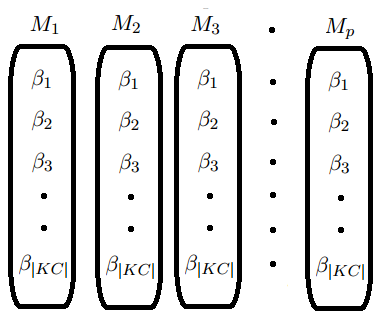
\includegraphics[width=.42\textwidth]{images/uitleg.png}
\end{center}
\caption{Experiment Schematic}
\label{fig:explain}
\end{wrapfigure}

The split is made by randomly distributing the students over the different parts. Each student is thus found in only one part and all questions belonging to that student are found in that part. This is done for a few reasons. First, this way of splitting keeps the data as much as possible in a grouping that can be seen in a dataset from an ITS.  Second, splitting the model according to KCs is more difficult as items can belong to multiple KCs. Also since there are more students than KCs, variance estimates for students would be more difficult as parts would more easily not contain any records of a single student. Finally, a practical matter, the count of how often a student has answered a question concerning a knowledge component is implicitly available in the data. Variance of the parameters that are defined per student are thus not obtained by this method, only variances for the the KC parameters.

In order to answer subquestion 1, splits with different numbers of parts are made. Five different splits are used with 6,8,12,16 and 32 parts. The splits with 6 parts have the most data and the splits with 32 parts have the least. It should be noted that a split with fewer parts has a higher second order variance for the found variance of parameters.

The found parameter variances are difficult to interpret due to a lack of a frame of reference for each model and parameter-type. To provide a frame of reference a model is fitted on the entire data-set. The variance within each parameter type of this model is used to normalize all the individual parameter variances found over the splits. In terms of Figure \ref{fig:explain} this means that of the model fitted on all data the variance over the column is calculated for each parameter-type and that the variance over each row is divided by this variance. By showing how the variance of parameters correspond to total variance within that parameter-type, variances of parameters of the same and different parameter-types and models can be interpreted and compared.

\subsection{Obtaining Variance of Orderings}
As put forward in subquestion 2, it is not always the exact values of the parameters that are of interest: sometimes the order of parameters is what is of interest. For these cases we are not interested in the variance of parameter, but rather the variance in the ordering of parameters within each parameter-type. Rank-order correlation measures are a good measure for these cases.

Rank-order correlation measures can be used to indicate how similar two orderings are. They take a set of paired values as input and return a single value. The paired values in our case would be a parameter value from one model and the same parameter (belonging to the same KC) value from another model. Rank orders are made for parameter-types from both models, meaning that every value is replaced with its rank (i.e. 1 for the highest value, 2 for the second highest). A correlation is then made between the two rank orders, where a value of 1 means that if the one value is the x highest value, the paired value in the other set is also the x highest value. A rank order correlation of -1 means the opposite: if one value is the x highest, the paired value from the other model is the x lowest value. In our example we would expect a positive rank order correlation value. Nevertheless we do not expect a value of 1 since we expect variance in the parameters to prevent the ordering from being exactly the same. 

For comparing two orderings of the same parameter-type we use Kendall's Tau (\cite{rank}). Kendall's Tau looks at all possible combinations of two elements from the set and looks whether or not the ordering of their paired values is the same. Formula \ref{eq:tau} shows the definition for Kendall's Tau, where $S$ is the number of tuples where the relation for both elements of the pairs is the same and $D$ where the relation is different. For example if we take the tuple $(\beta_{2},\beta_{5})$ and in our first model $(\beta_{2}>\beta_{5})$ and in our second model $(\beta_{2}<\beta_{5})$ this tuple would add one to D. $n$ is the number of paired values. The denominator in formula \ref{eq:tau} is then equal to the number of possible tuples within the set of values.
  
\begin{equation}
\label{eq:tau}
\tau=\frac{S-D}{\frac{1}{2} n (n-1)}
\end{equation}

The reason for using Kendall's Tau is that it indirectly serves as an accuracy measure for telling parameters apart. In only $\frac{\tau+1}{2}$ of the cases, a parameter that is greater than another parameter in one set of parameters, is also greater than that parameter in the other set of parameters. In the experiment there are as many models as there are parts. To obtain a single value for each parameter-type in an experiment the average $\tau$ value over every combination of two models in that experiment is calculated.

\subsection{Inherent Variance}
Inherent variance is used as the name for the variance caused by the stochasticity of the model. Variance caused by stochasticity of the model was already discussed for the IRT models and the same issue plays a role in data based on IRT as discussed in subquestion 4.

In section \ref{sec:inherent} information functions were mentioned and how they are used in IRT to establish lower bounds for variance. Here too we want to find out what minimum of variance is to be expected due to the stochasticity of the model, but in this case we need to fit both student and item parameters at the same time. We have not found a proper equivalent of an information function for the IRT-based learner models, thus a different approach is taken.

The situation described by Baker in section \ref{sec:inherent} can also be achieved by simulating the model. In the simulated approach, first the parameters are determined by fitting the model on the data (here the labels do have their influence on the result). The found parameters are then used to stochastically generate new labels for the data. This means that if the model predicts a .2 probability that the question is answered correctly, 20\% of the time the label will be 1 and 80\% of the time the label will be 0. In the PFA model this generated answer will also influence further probabilities due to the different learning rates for correct and incorrect answers to questions. Multiple sets (10 in our experiments) of labels are generated for the data in this fashion, after which the same model is fitted again on these sets. The inherent variance of every parameter is then estimated by calculating the variance of that parameter over the different trained models.

For subquestion 3, the influence of amount of data, the Kendall's tau value is also calculated between every pair of generated models to see how inherent variance changes the rankorder of parameters. The average $\tau$ value of all these pairs is used as a one metric to see the inherent invariability of the ordering of parameter values. 

In the experiment inherent variance and order variance are calculated for each part of every split, since the data in every part can be (very) different and thus have a large influence on the found inherent variances. The average of the variances and $\tau$ values is taken per split, so that they can be compared to the values found per split for the observed data. 

\subsection{Model Fit and Prediction Accuracy}
\label{sec:perf}
As can be seen in this section the methods used to obtain the variance of the parameters is complicated. This makes these methods time consuming  take quite some time and the available data is split into parts, making this method unable to make statements about variance of parameters when the whole dataset is used.  In the 5th subquestion the question is put forward if quality measures that are easier to obtain and already used to judge model quality, correlate with found invariability of the model parameters.

\subsubsection{A'}
The most common performance measure used in the context of ITS learning models is some measure of accuracy of model predictions on a test-set. The specific accuracy measure used for this research is A' (pronounced a-prime) \cite{modelreview}. A' uses a test-set, but it does not simply return the number of answers the model predicted correctly. Instead it makes every possible pair of questions of which one is answered correctly and one is answered incorrectly. The A' measure is the ratio of these pairs where the model gave the correctly answered question the highest probability of the pair of questions. The advantage of this method is that ``values of A' are statistically comparable across models and data sets" \cite{modelreview}.

In order to create a testset the last seven observations of every student are withheld as a test-set. This way of creating a test-set might skew the A' value towards poorer performance than if the last 10\% of observations for every student was taken, because poorer performance is expected for students of whom few questions have been observed, which now form a larger portion of the test-set. On the other hand taking the last 10\% of observations per student would favor models fitted on data where a few students answer the majority of questions. In the end either method is defensible and the method used should be taken into account when comparing A' values of datasets where a testsets were selected in a different way. When calculating the A' values for a part only those students who's questions are in that part of the data are used.

\subsubsection{Average Log Likelihood}
Log likelihood of the data given a model is another measure that plays a large role in this specific context as this is what is maximized in fitting the model. The log likelihood gives an idea of how well the model fits the data. Log likelihood is also used in the BIC and AIC criteria that are used in \cite{lfa} to judge model quality. Although these measures are preferable because they protect from simply favoring more complex models, the problem with these measures is that they cannot be compared when models are fitted to different datasets, especially when the amount of data differs as is the case here. To compare log likelihoods of models fitted on different sized data-sets, it will be normalized by dividing it by the number of data points. 

\subsubsection{Finding Correlations}
In looking for correlations between the above measures and the invariance of the parameters of the model we do not want to limit ourselves to a particular function to match both. Again a rank correlation measure will be used, since a good feature of a rank correlation value is that it can indicate whether there is a monotonic relation between the pair of values, without considering the fit of any specific monotonic function. 
 
The rank order measure used for this problem is Spearman's rho (\cite{rank}) (The word rho will be used rather than $\rho$ to distinguish it from the parameter). The formula for Spearman's rho is seen in formula \ref{eq:rho} Where $d_{i}$ is the difference in rank for the $i$th pair of values and n is the total number of pairs.
\begin{equation}
\label{eq:rho}
1-\frac{6 \sum\limits_{i=1}^n d_{i}^{2}}{n(n^{2}-1)} 
\end{equation}
The difference with Kendall's tau is that more emphasis is put on 'outliers' (large differences in ranks between pairs). This is done as outliers are more problematic in the case of judging which model is better.


\begin{comment}
\todo{currently this part is out of the question. I might bring up this discussion again:
Additionally a method that from IRT \cite{hambleton} will be used. After initially fitting the data will be split in two along student initial knowledge, such that one set contains all the lowest values and the other all the highest. Then the fitting will be done again on both new data-sets. If the assumptions of the model were correct the parameters for items should be roughly the same. It is expected though that this will not hold as there probably is a relation between having a high initial skill and how fast one learns knowledge components}

Although the primary way in which model parameters will be examined is described above, alternative methods will be used where applicable. Some data-sets contain additional information that can be used to more directly draw conclusions on whether found parameter values are meaningful. Two examples from the related research section are \cite{eirt} where expert opinions and an indication of what groups have higher initial knowledge were used and \cite{ktpfa} where a pre-test was used as an indicator of initial knowledge.
\end{comment}

\subsection{Data cleaning}
\label{sec:cleaning}
Splitting the data may exacerbate some of the issues that can be encountered in fitting the model. One example is when all questions associated with a student or a KC are answered correctly or incorrectly. This makes the fitting algorithm want to assign infinite values to parameters. Another problem is when for a KC there is such a limited number of questions answered that learning rates cannot be estimated: if there is never more than one question per student concerning a specific KC, the learning rate for this KC could have any value fitted to it.

To prevent these issues the following steps are taken. On the whole dataset, students that answer all questions correctly or incorrectly are removed. This is after having moved the last 7 questions per student to the test-set (used for A'), which means that any students who answered less than 9 questions were all dropped from the data. 
In every split, KC's for which every question is answered correctly or incorrectly is removed from that split. Additionally if for a KC there is not a student that  answered two questions correctly and who answered two questions incorrectly, that KC is not taken into account for that split. This means that this KC is removed from the items and any item that no longer contains a KC is dropped from the data. This is done iteratively until the data adheres to these conditions. How many KCs and students were left out in every split is represented in the results to show how big of an issue this was and what impact it might have on the results.

Note that this may have as an effect that for some KCs parameter values are only found in a few parts of a split. Parameters of KCs that are only found in less than 3 splits are left out of the results of the experiment as well. The number of KCs left out is displayed in the results section.


\subsection{Domains}
\label{sec:domain}
In fitting a model to the data there are many factors that might play a role in how invariant the parameters are. Among those factors are the values that the parameters have, the distribution of knowledge components over the items, the ratio of students to items, the quality of the cognitive model used, noise in the data etc. As indicated in Section \ref{sec:RQ} these factors are not explored methodically and extensively, but rather a few different datasets are used to represent some of the variation naturally found in this kind of data. A short description of where these datasets come from are given below. In Table \ref{tab:datdat} some statistics are given for each dataset. The number of questions is equal to the total number of data-points used for fitting the models after taking out the test-set and doing an initial cleaning. The number of knowledge components and students show how many were removed from the dataset and how many still remain. Only a cleaning sweep over the entire data is taken into account here. Information on how many KCs and students were dropped due to the making of splits is given in the results section. Table \ref{tab:QKC} counts for each number of associated KCs, how many questions are asked in each dataset. This was chosen over showing the number of items per number of associated KCS, since in the data the distribution of how how often items are seen is skewed. 

\subsubsection{Bridge to Algebra}
The first data-set is one of the datasets used in the 2010 KDD cup on education data mining. The data is from Carnegie Learnings' Cognitive Tutor Software meant for high school-students aged 15-18. \cite{ct} provides an overview of some of the features of this program. The data was obtained from the Bridge to Algebra course during the school year 2006-2007 \cite{bridge}. This dataset will be referred to as the Bridge dataset.

\subsubsection{Algebra I}
This dataset was also provided in the 2010 KDD cup. The data is also obtained from Carnegie Learnings' Cognitive Tutor Software, but from the Algebra I course during the school year 2005-2006 \cite{algebra}. This dataset will be referred to as the Algebra dataset.

\subsubsection{Assistment}
This dataset is quite different from the other two as it is taken from a web-based ITS named Assistment whose details and development story can be found in \cite{razzaq}. The data is from 12 to 14 year old students and was used in \cite{ktpfa} which was discussed in section \ref{sec:RW}. The data does not only contain data from usage of the ITS but also data from a pre-test. This dataset will be referred to as the Assistment dataset.

\begin{table}
\centering
    \begin{tabular}{| l | l | l | l |l|l|}
    \hline
    Dataset & \# questions & \# KCs(removed) &\# students(removed) & \% correct(testset)&\# items \\ \hline
    Bridge & 1,814,398 & 455(34) & 1129(17) & 83(80)& 129,553 \\ \hline
    Algebra & 585,557 & 104(6) & 564(10) &  76(75)& 173,650\\ \hline
    Assistment & 110,842  & 106(0) & 425(20) & 65(59)& 807\\
    \hline
    \end{tabular}
    \caption{Basic information on each dataset}
    \label{tab:datdat}
\end{table} 
   
\begin{table}
\centering
	\begin{tabular}{| l | l | l | l |l | l |}
    \hline
    Dataset & 1 & 2 & 3 & 4 & 5-7\\ \hline
    Bridge & 1801254 (0.993) & 11406 (0.006) & 1623(0.001)&113(0.000)&2(0.000) \\ \hline
    Algebra & 368875(0.630)  & 114600 (0.196) & 85818 (0.147)&5581 (0.010)&10683 (0.018) \\ \hline
    Assistment & 56521 (0.510) & 37356 (0.337) & 11770 (0.106) & 4237 (0.038)&958 (0.009)\\
    \hline
    \end{tabular}
    \caption{How often questions have a particular number of KCs associated with them. The proportion of the total is given in brackets}
    \label{tab:QKC}
\end{table}  

\begin{comment}
2(0.000)& 0&0
6455 (0.011)& 4123(0.007)&105(0.000)
958 (0.009)&0&0
\end{comment}


\subsection{The Experiment}
In detail the experiment for KC parameters consists of the following steps:
\begin{enumerate}
\item Train a 'main-model' on the whole dataset
\item Clean the data by removing students according to section \ref{sec:cleaning}
\item Split the data in a number of parts. Then for each part:
\begin{enumerate}
\item Clean the data by removing KCs according to section \ref{sec:cleaning}
\item Train the model on the part
\item Determine performance on the test-set for that split
\item Determine the average inherent variance through simulation
\item Determine the average Kendall's tau value over all model trained on simulated models (=inherent tau)
\end{enumerate}
\item Determine the variance per parameter over all the parts
\item Determine the average Kendall's tau value between all the model
\item Determine the average inherent variance and Kendall's tau over all parts 
\item Normalize all the found variances with the variances per parameter-type from the main-model
\end{enumerate}

The experiment is done for every combination of split (6,8,12,16 and 32), model (LFA, PFA+ and meIRT) and dataset (Bridge, Algebra and Assistment). In total this results in 5x3x3=45 experiments being performed.


\section{Results}

 
\begin{wrapfigure}{R}{.25\textwidth}
\begin{center}
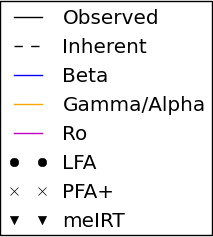
\includegraphics[width=.24\textwidth]{images/legend.png}
\end{center}
\caption{Legend for all figures in this section}
\label{fig:legend}
\end{wrapfigure}





\subsection{Left Out Knowledge Components}
In section \ref{sec:cleaning} it was described that some KCs are removed in order to fit proper models. Removing data directly impacts the conclusion because KCs that are left out in this way would have a (relatively) high variance if there had been a little more data for them so that they could have been left in. To investigate the extent to which KCs are left out this section reports on how many KCs were left out.   

In Table \ref{tab:kcmis} it can be seen how many KCs were missing on average over the experiments using the different models (the splits were remade for every model). The number outside brackets is how many KCs were left out of that experiment completely (i.e. no standard deviation is calculated for them). The number between brackets indicates how many KCs were on average missing from each part in the experiments for that split, including those that were left out of the experiment in the end (i.e. the other were left out of some of the parts, but still enough parts remained to calculate a standard deviation over them). 


\begin{table}[h]
\centering
\begin{tabular}{| l | l|l|l|l|l|}

    \hline
    Splits & 6  & 8 & 12 & 16 & 32 \\ \hline
    Bridge &  87.3(90.1)& 85.7(99.7)& 88.0(121.2)& 87.7(137.1)& 89.3(190.4) \\ \hline
    Algebra & 7.3(8.5)& 6.7(8.9)& 6.7(11.5)& 7.0(14.0)& 7.7(21.3) \\ \hline
    Assistment & 0.7(1.2)& 0.7(1.1)& 1.0(1.3)& 1.0(1.8)& 1.0(5.7) \\ \hline

\end{tabular}
\caption{Average number of KCs left out of experiments with the average number of removed KCs per split within brackets}
\label{tab:kcmis}
\end{table}


The number of KCs left out is almost constant for each dataset; the increasing number of KCs missing per part as the parts get smaller is apparently off-set by the increasing number of parts. It does mean though that the second order variance of variances found would be higher than expected.

The number of KCs left out per dataset follows the same distribution of KCs left out per dataset in the initial cleaning which was seen in Section \ref{sec:domain}: Many KCs are left out of the Bridge datasets, less from the Algebra dataset and least for the Assistment dataset. For the Bridge dataset the KCs removed (including those removed before the experiments) form almost 25\% of the total KCs. Although it is unfortunate to miss this much data, it shows that for many KCs in this dataset little data is available and that average variance of parameters would probably be worse when these KCs would be included. For the Algebra dataset the problem is smaller, but still substantial (12\% of KCs are left out). Only for the Assistment dataset this problem is almost non-existent (<1\%).

\subsection{Orderings within parameters}
\label{sec:rankresults}


To answer subquestion 2, ``What is the variability of the orderings within the KC parameter-types?", Kendall's tau values were calculated over the parameter-types of different models build within each experiment. In Figure \ref{fig:ranks} the resulting average $\tau$ values can be seen from all the experiments (see Figure \ref{fig:legend} for the legend of this and all following figures). A $\tau$ value of .5 is considered here as a reasonable $\tau$ value for a parameter-type order to be invariant. At this $\tau$ value 75\% of the pairs of parameter values would still be in the same order between two different fitted models.



Even at the highest amount of data used the $\rho$, $\gamma$ and $\alpha$ parameter-types never have a $\tau$ value of .5 or greater. The orderings of these parameter-types are so variable that they should be disregarded. The $\rho$ parameters of the PFA+ models show particularly low $\tau$ values which show that the orderings of these parameter values are near random.



The $\beta$ parameter-type of the PFA+ and LFA models do not always have a $\tau$ above .5 at lower amounts of data, but as data is increased $\tau$ increases above .5 for both models on all datasets. The $\beta$ parameter-type of the meIRT model $\tau$ does come above .5, but only for two of the datasets and at the highest amounts of data. For the Algebra dataset $\tau$ of the $\beta$ parameter-type is always well below .5. The $\beta$ parameter-type ordering of the PFA+ and LFA models is generally sufficiently invariant, while for the meIRT model it is mostly too variant.


\begin{figure}[h]
\centering

\subfloat[Ordering variance results for all experiments on the Bridge dataset]{
  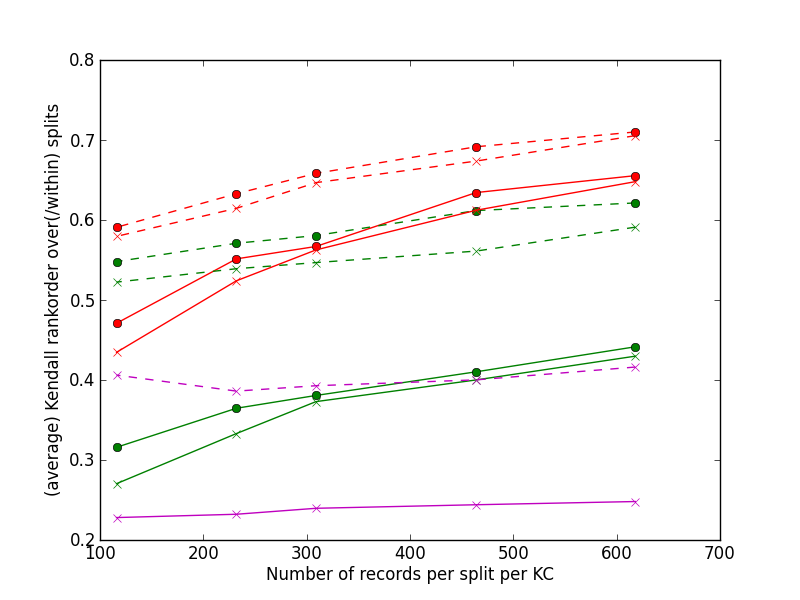
\includegraphics[width=70mm]{images/bridgeallmodranksKC.png}
}
\hspace{0mm}
\subfloat[Ordering variance results for all experiments on the Algebra dataset]{
  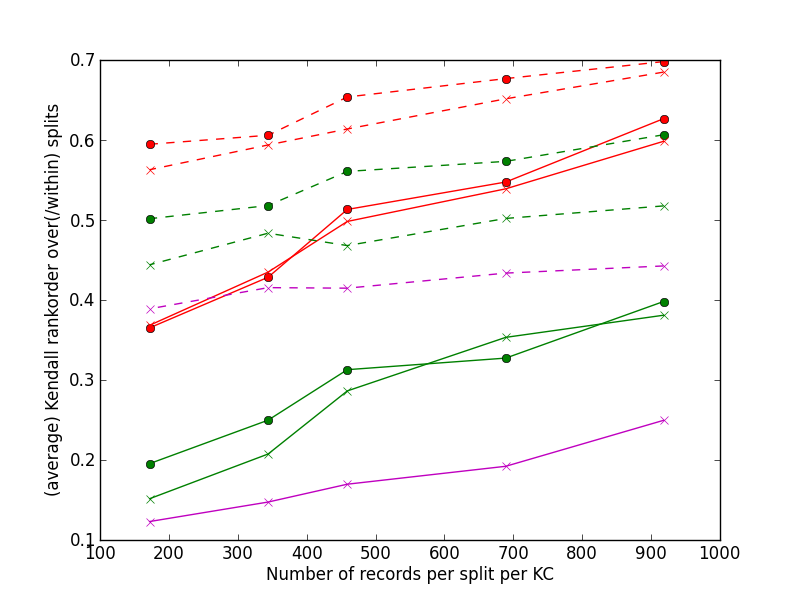
\includegraphics[width=70mm]{images/algebraallmodranksKC.png}
}
\hspace{0mm}
\subfloat[Ordering variance results for all experiments on the Assistment dataset]{
  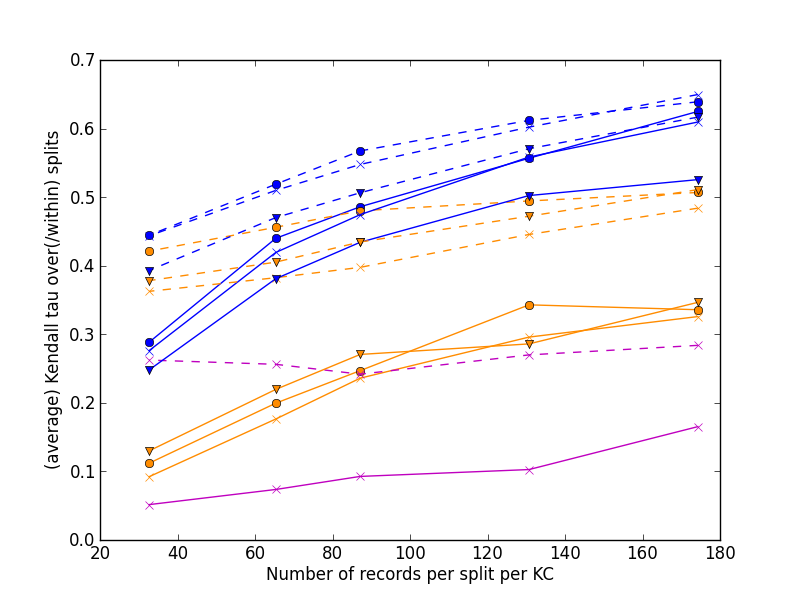
\includegraphics[width=70mm]{images/gongallmodranksKC.png}
}
\caption{Kendall's Tau rank orders of the different parameter-types}
\label{fig:ranks}
\end{figure}




\begin{comment}
\begin{wrapfigure}{r}{.7\textwidth}
\begin{center}
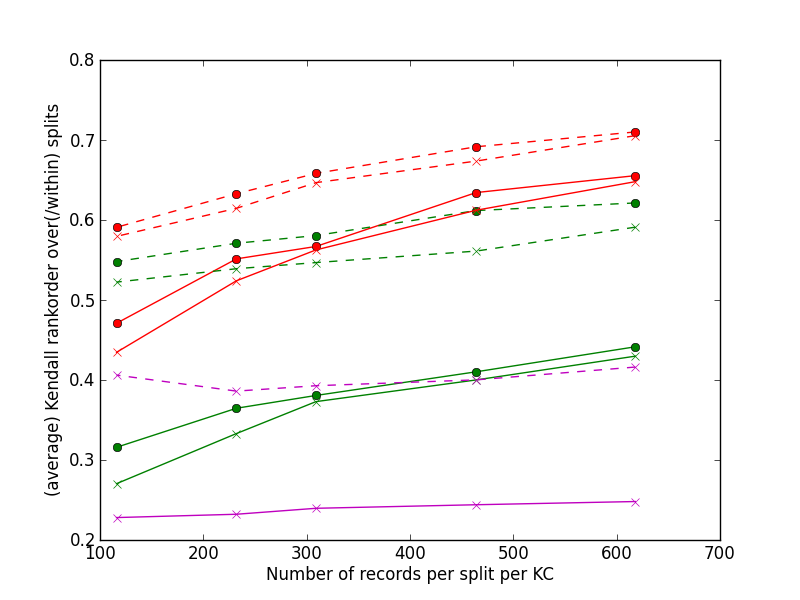
\includegraphics[width=.7\textwidth]{images/bridgeallmodranksKC.png}
\end{center}
\caption{Ordering variance results for all experiments on the Bridge dataset}
\label{fig:legend}
\end{wrapfigure}

\begin{wrapfigure}{l}{.7\textwidth}
\begin{center}
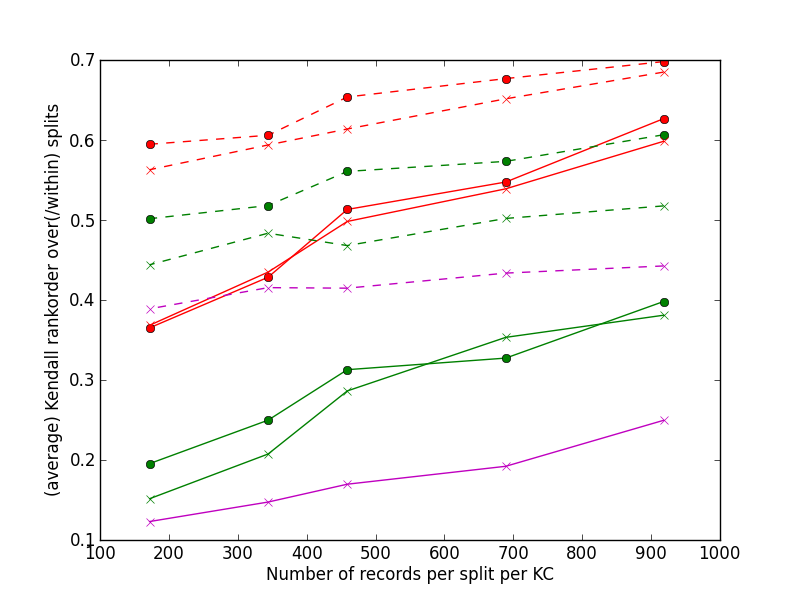
\includegraphics[width=.7\textwidth]{images/algebraallmodranksKC.png}
\end{center}
\caption{Ordering variance results for all experiments on the Algebra dataset}
\label{fig:legend}
\end{wrapfigure}

\begin{wrapfigure}{r}{.7\textwidth}
\begin{center}
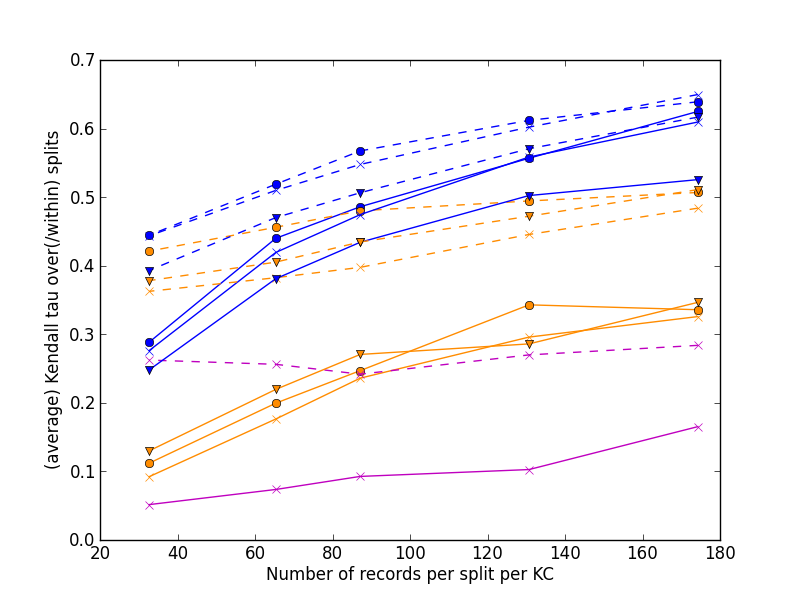
\includegraphics[width=.7\textwidth]{images/gongallmodranksKC.png}
\end{center}
\caption{Ordering variance results for all experiments on the Assistment dataset}
\label{fig:legend}
\end{wrapfigure}

\end{comment}


The conclusion here is that the LFA and PFA+ models' learning parameters ($\gamma$ and $\rho$) cannot be well distinguished from other parameters of the same type and that these models can provide too little information about relative learning speed of different KCs. The same goes for the $\alpha$ parameters of the meIRT model. The effects of this might be far reaching as this parameter-type augments the initial knowledge and learning parameters in application of the model. The $\beta$ parameters of the LFA and PFA+ models score sufficiently on distinguishability, except in the cases where the lowest amount of data was used. The $\beta$ parameters of the meIRT model do worse than those of the LFA and PFA+ models and proved to only be sufficiently distinguishable in the experiments on the Bridge and Assistment datasets where the maximum amount of data was used.  

Figure \ref{fig:ranks} also holds information for the third subquestion, ``What is the influence of the amount of data on invariability?". In this case it specifically concerns the invariability of parameter rank orders within parameter types. The hypothesis that invariance increases as more data is used holds except for a few minor exceptions that might be ascribed to noise. When looking in detail to relationships over all datasets there seems to be no direct relation between the number of records per KC used and the $\tau$ value, failing to give a rule of thumb for how much data is needed. An alternative measure of amount of data might be successful. The alternatives of looking at students per KC per split and students per split was considered, but in the first case the Bridge datasets would obtain low values and the last option would leave the Bridge dataset with high values compared to the other two, while the $\tau$ values are comparable. A possible cause of the differences might be found in structural differences in the data, for example that number of records per KC is more evenly distributed in the Assistment dataset than in the others.  

Finally, Figure \ref{fig:ranks} provides information for the fourth subquestion, ``To what extent is variability expected given the stochasticity of the model?". The hypothesis was that the variability of the observed parameter orderings is always worse than the variability of parameter orderings in generated data. This hypothesis holds everywhere and thus the inherent variability obtained through simulation can serve as a lower bound for the variability of the actual parameter orderings. 


\subsection{Overall Invariance of Parameters}
\label{sec:varresults}
\subsubsection{Overall Variance}
To answer the first subquestion, ``What is the standard deviation of the KC parameter values?", the average standard deviation of parameters per parameter-type is displayed in Figure \ref{fig:sds} for all experiments. As described in Section \ref{sec:splits} the values are normalized by dividing them by the standard deviation within the values of that parameter-type in a model fitted on the whole dataset. This way standard deviations of different parameter-types can be compared to each other and the presented value is easier to interpret. 

\begin{figure}[h]
\centering
\subfloat[Average standard deviations for all experiments on the Bridge dataset]{
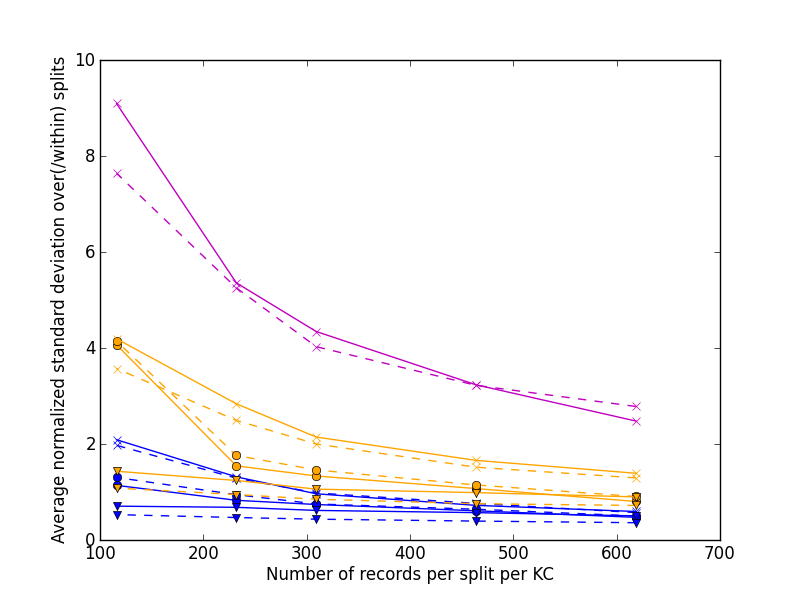
\includegraphics[width=70mm]{images/bridgeallmodsdsKC.png}
}
\hspace{0mm}
\subfloat[Average standard deviations for all experiments on the Algebra dataset]{
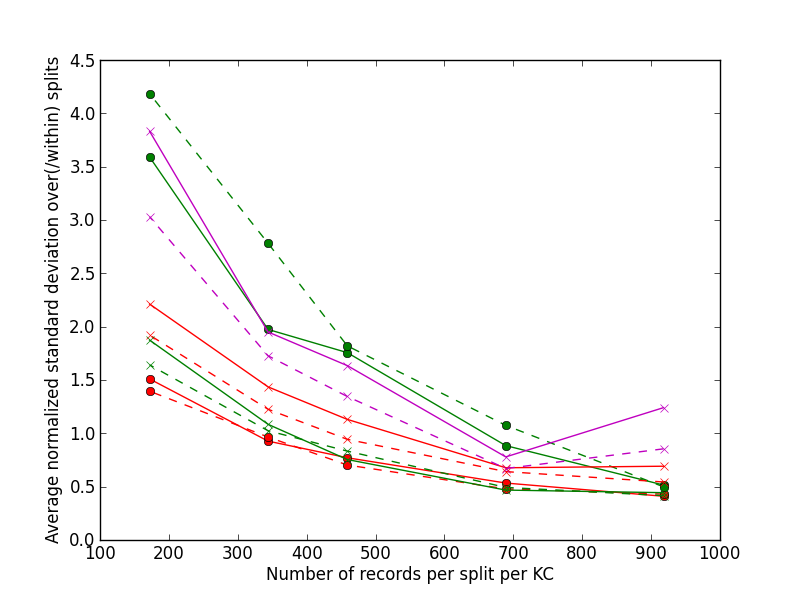
\includegraphics[width=70mm]{images/algebraallmodsdsKC.png}
}
\hspace{0mm}
\subfloat[Average standard deviations for all experiments on the Assistment dataset]{
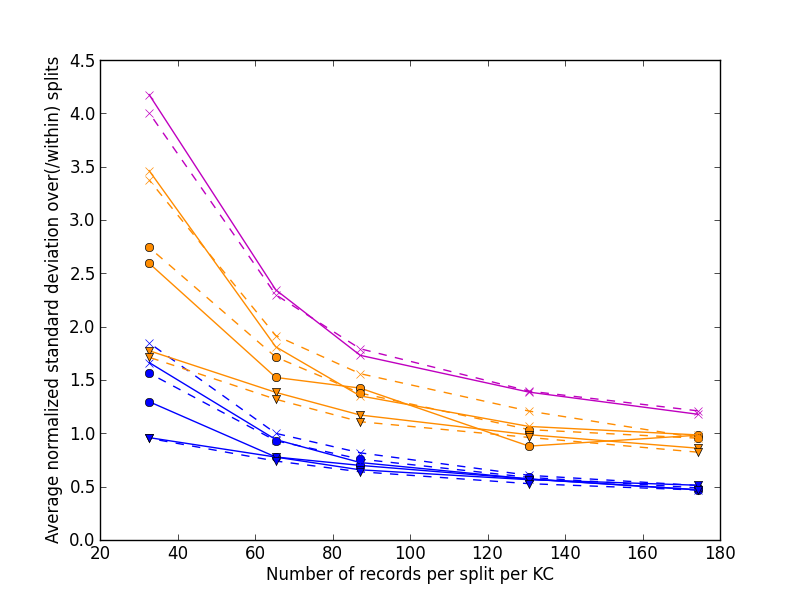
\includegraphics[width=70mm]{images/gongallmodsdsKC.png}
}
\hspace{0mm}
\caption{(Average) standard deviations of the different parameters}
\label{fig:sds}
\end{figure}

At first glance these results correspond to the results from the previous section. A few point are suspicious though: 1. the normalized variance, especially at splits where the parts have fewer data is extremely high 2. The difference between inherent variance and observed variance is generally low, while in the previous section the differences between the rankings were clear. 3. The ratio of variance of the parameters and the variance within a parameter-type should not be higher than 1. Investigating this problem let to the discovery that standard deviation within the parameter-types differs between the models fitted on the whole datasets and those fitted in the experiments. The following subsection investigates this issue in more detail.


\subsubsection{Standard Deviation within Parameter-types}
\label{sec:parvar}
In order to see how the standard deviation of the parameter-types differ between the models fitted in the different experiments and the models fitted on the whole datasets, Figure \ref{fig:parvar} displays the average standard deviation within the parameter-types in those experiments relative to the standard deviation within those parameter-types in the model fitted on the whole dataset. In terms of Figure \ref{fig:explain} this means that the average of the standard deviation of every column is taken and divided by the standard deviation over the column of the model fitted on the whole data. Since these standard deviations also differ between models fit on observed data and those fit on generated data these variances have been determined separately and divided by the same standard deviations. Due to the large values for some parameters, especially at parts with little data, a zoomed in version is displayed in Figure \ref{fig:parvarz}. 
\begin{figure}[h]
\centering

\subfloat[Standard deviations within parameter-types for the Bridge dataset]{
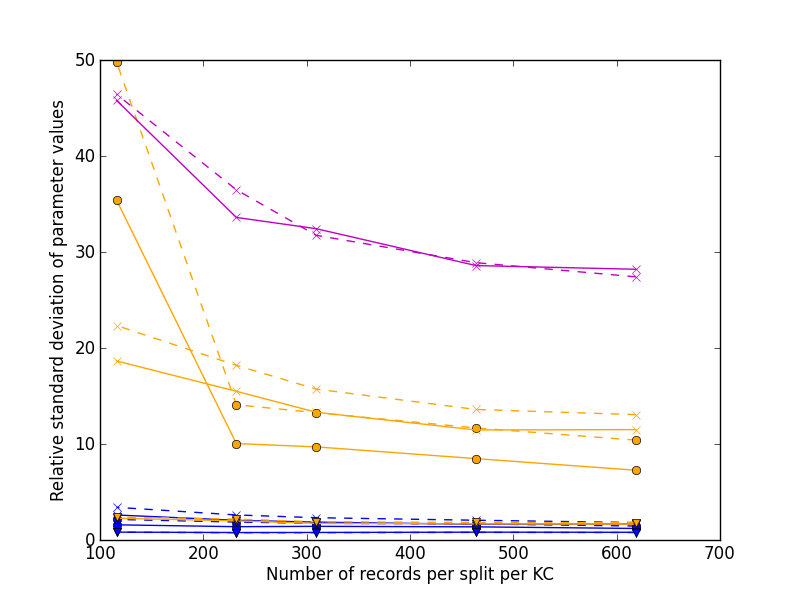
\includegraphics[width=70mm]{images/bridgeallmodsparvar.png}
}
\hspace{0mm}
\subfloat[Standard deviations within parameter-types for the Algebra dataset]{
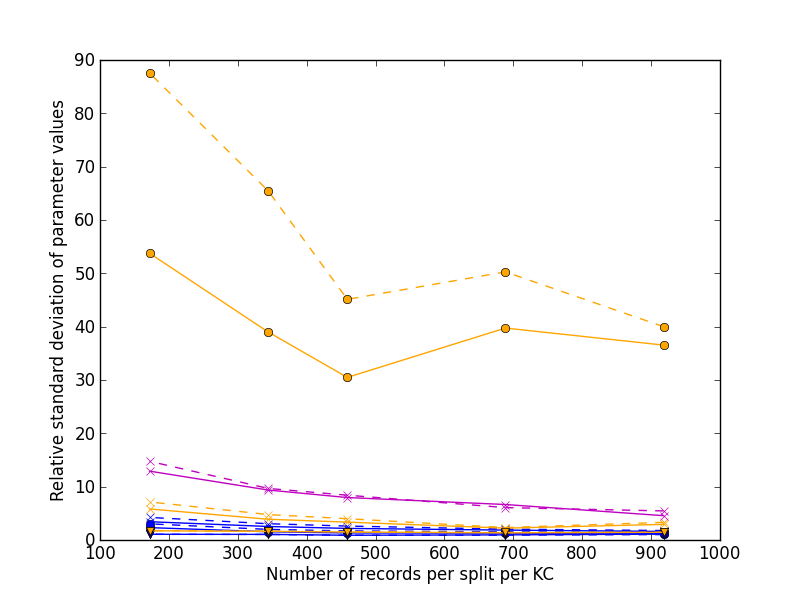
\includegraphics[width=70mm]{images/algebraallmodsparvar.png}
\label{fig:parvaralg}
}
\hspace{0mm}
\subfloat[Standard deviations within parameter-types for the Assistment dataset]{
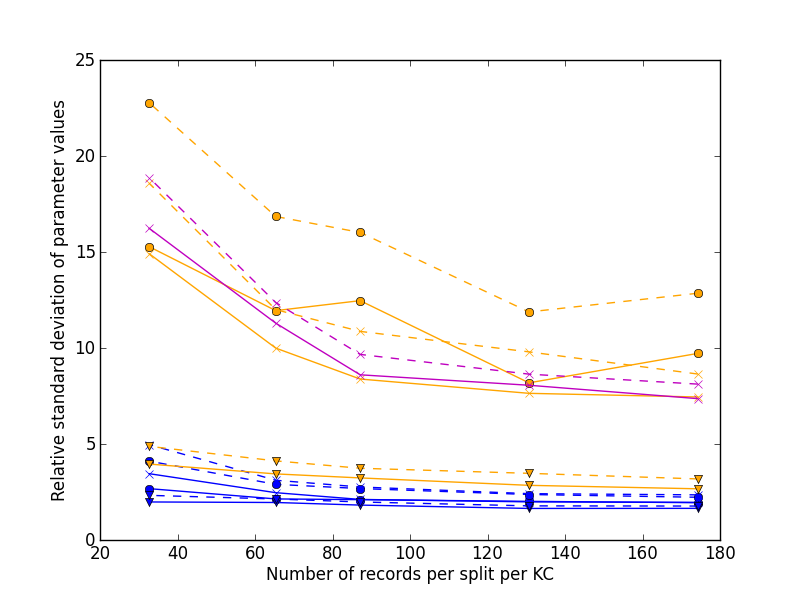
\includegraphics[width=70mm]{images/gongallmodsparvar.png}
}
\caption{(Average) standard deviations of the different parameters}
\label{fig:parvar}
\end{figure}

The standard deviations within parameter-types is lower when more data is used and indicates that the absolute values for these parameters are higher when less data is used. Even if the average standard deviation of parameters in an experiment is acceptable, changing magnitudes of the values for the same parameters over different experiments also means that these parameters are not invariant. Taking a cut-off value is more difficult here than it is for $\tau$ values: the interpretation of the value is less clear. Here a relative difference of having twice as large a standard deviation within a parameter-type compared to the standard deviation in the model fitted on all the data is still considered acceptable. Note that it is possible that the standard deviation within a parameter-type continues to fall if data were increased beyond the size of the full dataset. In the case when there is at max a two fold increase when the data is increased at least six fold (from 6 parts to a single part), it seems reasonable that not much decrease will be seen beyond this point.

In Figure \ref{fig:parvar} the high relative standard deviation within the learning parameter-types of the PFA+ and LFA models stand out. All the values of these parameters are well above the cutoff point. A possible explanation for these results is overfitting: if for example a question for a KC is answered wrong a few times early on by some students, but mostly answered correctly after those initial questions, the model will fit a very high learning rate to this KC. If more students would be present whom might continue to sometimes answer questions concerning this KC wrongly, the KC would be fitted a substantially lower learning rate value.

\begin{figure}[h]
\centering

\subfloat[Standard deviations within parameter-types for the Bridge dataset]{
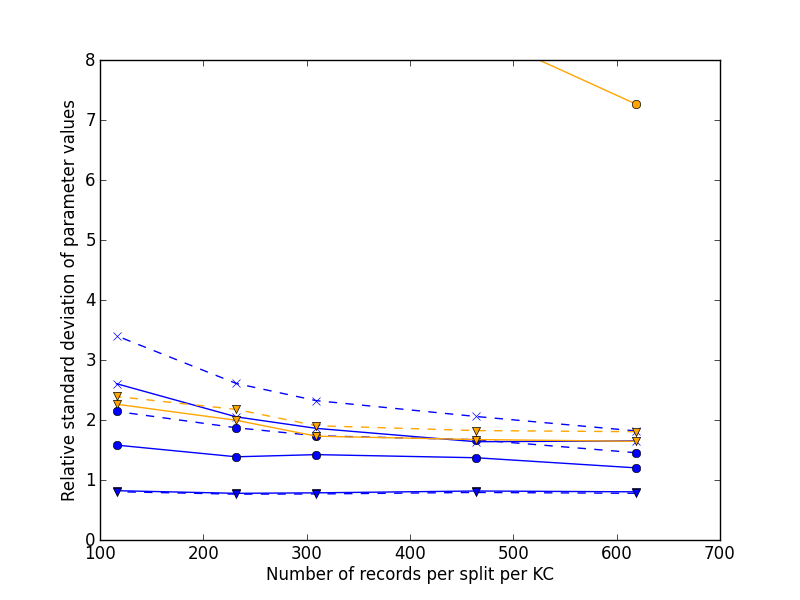
\includegraphics[width=70mm]{images/bridgeallmodsparvarz.png}
}
\hspace{0mm}
\subfloat[Standard deviations within parameter-types for the Algebra dataset]{
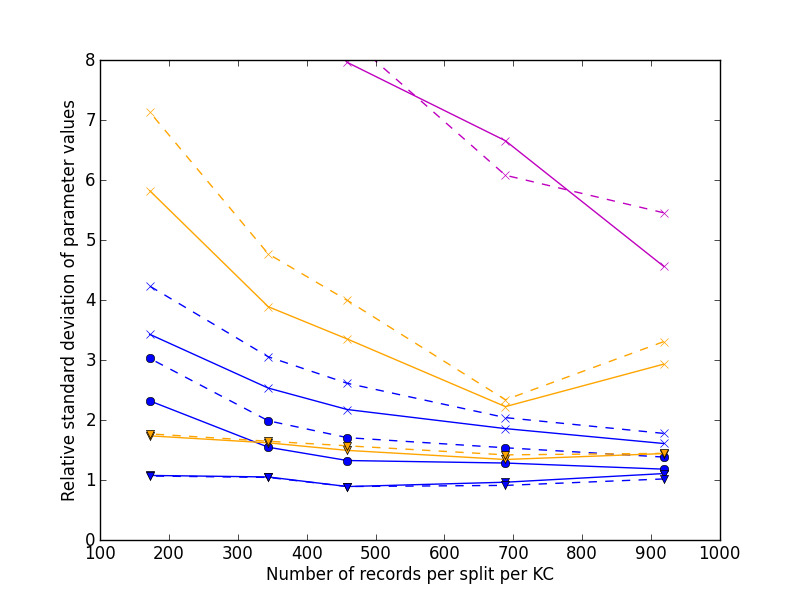
\includegraphics[width=70mm]{images/algebraallmodsparvarz.png}
}
\subfloat[Standard deviations within parameter-types for the Assistment dataset]{
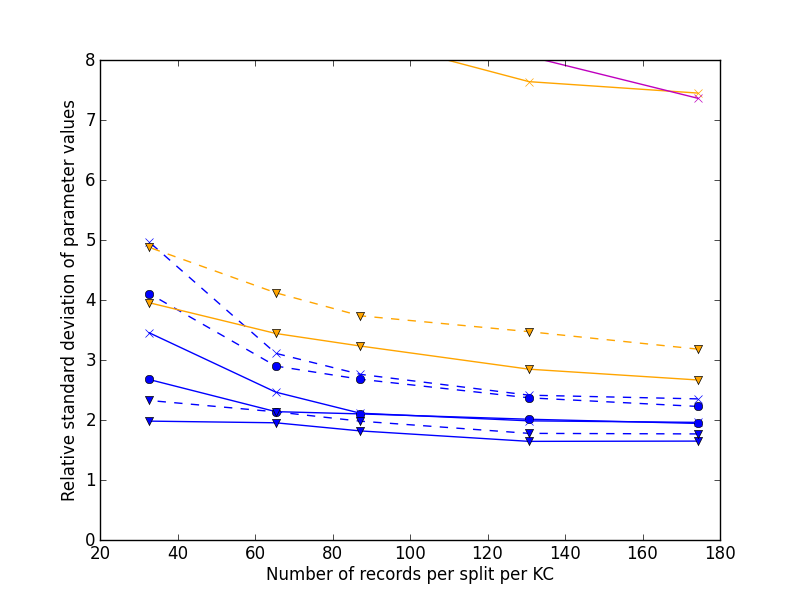
\includegraphics[width=70mm]{images/gongallmodsparvarz.png}
}
\caption{(Average) standard deviations of the different parameters}
\label{fig:parvarz}
\end{figure}

The $\beta$ parameter-types of the LFA, PFA+ and (especially) the meIRT models do better. At the experiments with the most data, the relative standard deviation within the $\beta$ parameter-types is below 2 at least at the experiments where most data is used for some datasets. Although all models do well enough in this regard the meIRT does best and the LFA model does better than the PFA+ model. Finally the $\alpha$ paramater-type of the meIRT model never reaches below 2 in experiments on the Assistment dataset, while being below in all experiments on the Algebra dataset and almost all experiments on the Bridge dataset.  

With regard to our investigation into the inherent invariability, it should be noted that the standard deviations for LFA and PFA+ models fitted to generated data are consistently higher than for those fitted on observed data. A possible explanation for this could be that overfitting continues to be a problem here, further increasing the size of parameters. Whichever is the case it weakens the basis of using simulated data to look at the theoretical variability of the parameters. meIRT shows the advantage of showing little difference between the two.

Finally there is an anomaly visible in figure \ref{fig:parvaralg}: the $\gamma$ parameter-type of the LFA model has high standard deviations, but the $\gamma$ and $\rho$ parameters of the PFA+ model do not. It would be expected that if the $\gamma$ parameters of the LFA model the are actually overfitted, the $\gamma$ and $\rho$ parameters of the PFA+ model, with even less data per parameter, would be overfitted as well. A possible explanation might be that in the LFA model the $\gamma$ parameter is fitted both high and low values, leading to a high standard deviation. In the PFA+ model high values are fitted mostly on the $\gamma$ parameters and low values on the $\rho$ parameters, resulting in lower standard deviations over both these parameter-types.

In conclusion the learning parameter-types of the LFA and PFA+ models are too variant, as the standard deviation over these parameter-types changes too much with the amount of data used. For the other parameters the results are better, although the details of why the standard deviations are higher should be looked into to establish if this cutoff point was correct. At any rate this problem obscures the obtained standard deviation values in Figure \ref{fig:sds}. These results are therefore not further used to answer the first subquestion, ``What is the standard deviation of the KC parameter values?".

\begin{comment}
\subsubsection{Adapted Normalization}
To account for the phenomena of increasing parameter sizes and still look at the standard deviation of parameters figure \ref{fig:sds} is repeated in figure \ref{fig:sdsalt}, but instead of using the variance in parameter-types of the model fitted on the whole data, the raw values from figure \ref{fig:parvar} are used to normalize the raw variances. This means that every datapoint has its own normalization factor instead of a single normalization factor for both the internal and observed variances of a model parameter at all different splits.

\begin{figure}[h]
\centering
\subfloat[Legend for the figures]{
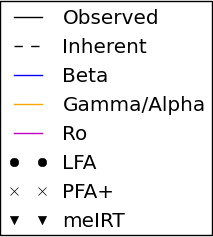
\includegraphics[width=30mm]{images/legend.png}
}
\subfloat[Standard deviations for Bridge parameters]{
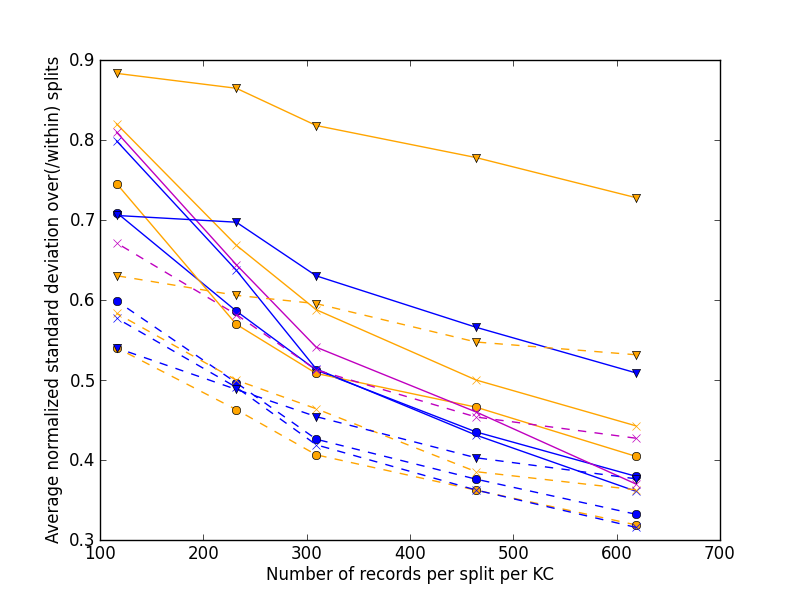
\includegraphics[width=65mm]{images/bridgeallmodsdsKCalt.png}
}
\hspace{0mm}
\subfloat[Standard deviations for Algebra parameters]{
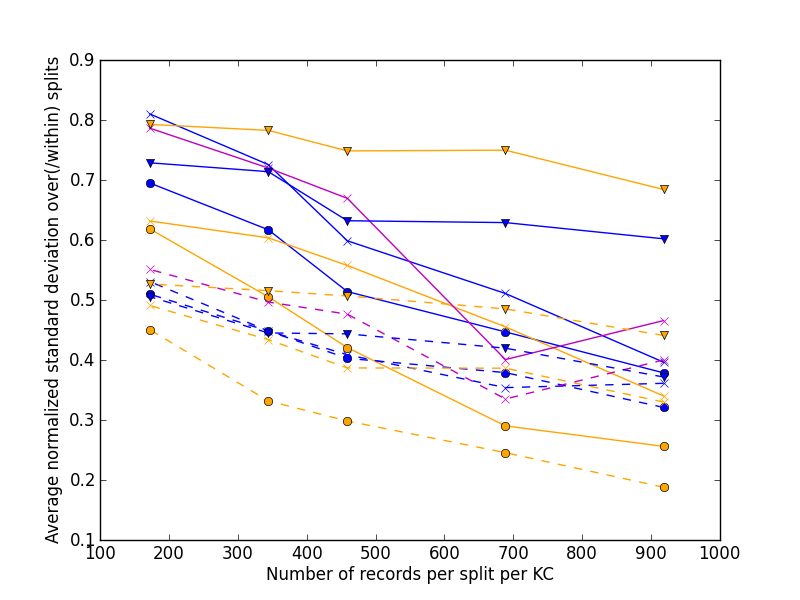
\includegraphics[width=65mm]{images/algebraallmodsdsKCalt.png}
}
\subfloat[Standard deviations for Assistment parameters]{
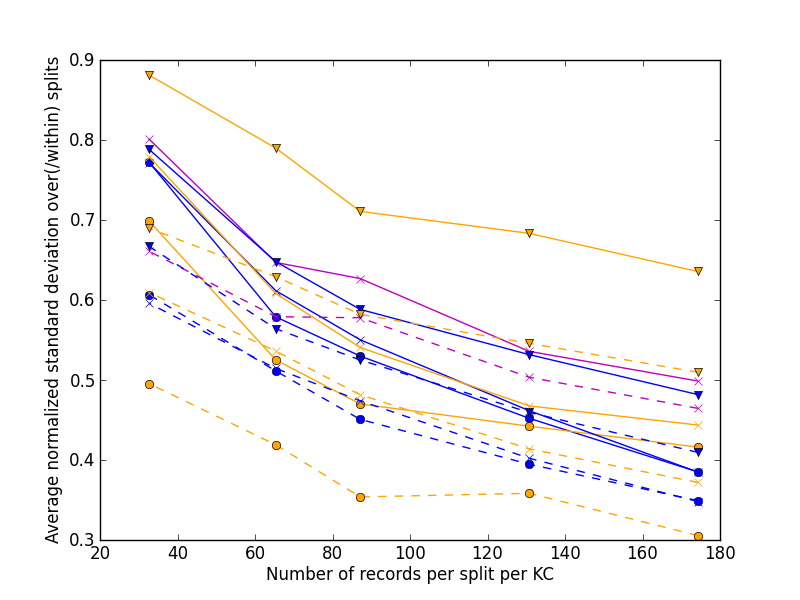
\includegraphics[width=65mm]{images/gongallmodsdsKCalt.png}
}
\caption{(Average) standard deviations of the different parameters}
\label{fig:sdsalt}
\end{figure}

In figure \ref{fig:sdsalt} the standard deviations of the parameters of the meIRT model are strikingly high. This is surprising since the $\tau$ values of this model aren't as bad. These contradictory results actually reinforce one of the reasons for using $\tau$: the normalization step of the models parameters in the fitting procedure increase the found variance, while not meaning that the model is necessarily worse.

The discrepancy between figure \ref{fig:sdsalt} and the found $\tau$ values doesn't stop at the meIRT model. The $\beta$ parameters of the other models also seem to be doing relatively worse compared to the learning parameters of these models. The conclusions form this observation is that this method is biased towards parameter-types with high standard deviations. This conclusion is futher considering that in the Algebra dataset the $\gamma$ parameters of the LFA model scores well on this metric compared to the other parameters, while this parameter-type also had a high standard deviation. This section thus brings to light some major problems with parameter invariability of the AFM and PFA+ models, but fails to supply other useful information.
\end{comment}

\subsection{Correlation with Accuracy and Model Fit}
To answer the fifth subquestion, ``Is the variability of the model correlated to prediction of accuracy and model fit?", only the $\tau$ values will be considered as measures of invariance of the models, because the average standard deviations of parameters were discarded in the previous section.

%As an exploration into the problem the average log likelihood values and the A' values of each experiment are plotted against the tau values of each parameter-type from the different experiments.  

\subsubsection{Average Log Likelihood}
In Figure \ref{fig:likely} the average log likelihood of the data is plotted against the $\tau$ values of the parameter-types from the different experiments. The points belonging to the different splits can easily be distinguished: there are three groups, one for each data set (from left to right, Assistment, Algebra and Bridge) and within each group the point with the highest $\tau$ value is the one with the most data associated with it. That the PFA models have a higher likelihood is to be expected as it has more parameters than the LFA models. It is also sensible that with more data in a split the likelihood goes down, since the increase in parameters (due to more students) is smaller than the increase in data. Although there is a visible relationship between $\tau$ and likelihood within each dataset, this relationship probably stems from the previous two relationships mentioned: as the amount of data goes up, so do the $\tau$ values and as the amount of data goes up, the likelihood goes down. When looking over all three datasets combined there actually seems to be a slightly positive relation between the average likelihood and $\tau$ values. The wide spread of $\tau$ values over splits of the same dataset (where the relation is quite negative) compared to the slight positive relation makes it unlikely that likelihood can be used to make inferences about the distinguishability of parameter values.
\begin{figure}[h]
\centering
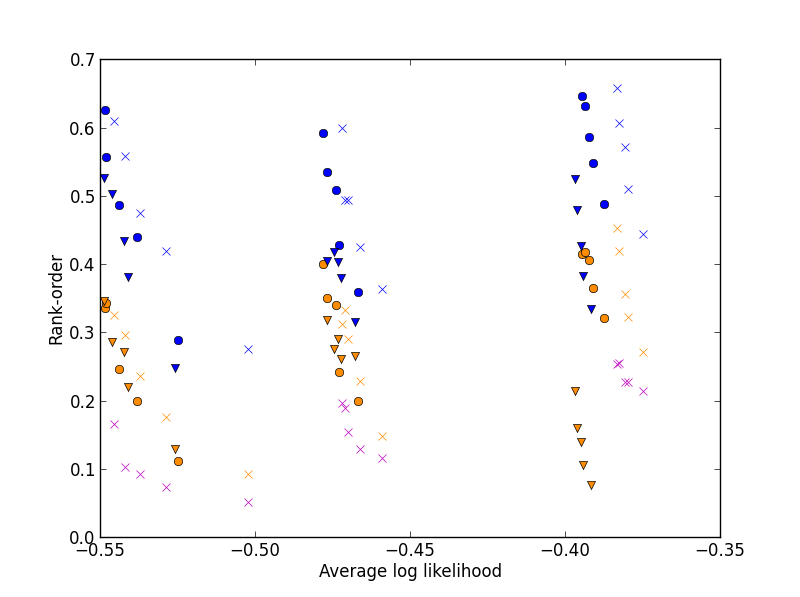
\includegraphics[width=140mm]{images/alllikely.png}
\caption{Average Log Likelihood vs Parameter-Type order Invariance}
\label{fig:likely}
\end{figure}

Table \ref{tab:cor} presents the Spearman's rho values between the likelihoods and $\tau$ values of each parameter-type in order to show the correlation between the two. Since quite a few values were high, which seems odd compared to Figure \ref{fig:likely}, Kendall's tau was calculated as well.  Kendall's tau gives more conservative estimates (which are also more easily interpreted) and is thus preferred after all. The $\tau$ values confirm our observation from Figure \ref{fig:likely} that no strong monotonic relation between likelihood and invariability of the parameter-type orderings exists.
%The reason why Spearman's r does better might be that there are 


\begin{table}[h]
\centering
\begin{tabular}{| l || l | l ||l|l |l||l|l|}

    \hline
     & LFA  & & PFA+ & & &meIRT &   \\ \hline
     & $\beta$ & $\eta$ & $\beta$ & $\gamma$ & $\rho$ & $\beta$ & $\alpha$  \\ \hline
    $\bar{LL}$     & 0.11(-0.01) & 0.40(0.22) & 0.05(-0.01) & 0.29(0.12) & 0.70(0.39) & -0.29(-0.26)&-0.71(-0.62) \\ \hline
    A'             & 0.75(0.58) & 0.86(0.73) & 0.64(0.54) & 0.82(0.71) & 0.94(0.83) & -0.05(-0.10)&-0.35(-0.24) \\ \hline

    \hline
\end{tabular}
\caption{Spearman's rho of `$\tau$ of parameter-types' vs. likelihood and A' (Kendall's tau in brackets)}
\label{tab:cor}
\end{table}


\subsubsection{A'}
In Figure \ref{fig:ap} A' is plotted against the $\tau$ values of the parameter-types from the different experiments. There seems to be a positive relation between A' and the $\tau$ of each of the different parameter-types in both models. From Table \ref{tab:cor} it turns out this suspicion is not true for the meIRT model and that the relation is less strong for the $\beta$ parameters of the LFA and PFA+ models.

\begin{figure}[h]
\centering
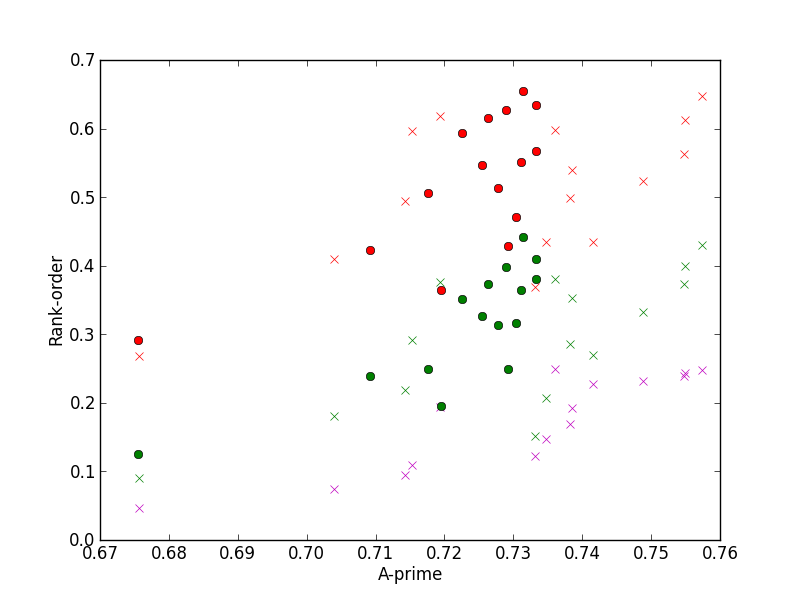
\includegraphics[width=140mm]{images/allaprimes.png}
\caption{A' vs Parameter-Type order Invariance}
\label{fig:ap}
\end{figure}

Finally a caveat: these results are per model, i.e. while comparing a LFA model to a LFA models, a higher A' is related to more invariant parameter-type orderings. When comparing different models this does not hold though. In Figure \ref{fig:ap} it shows that the A' values of the PFA+ model are higher than those of the LFA model, while we have seen in section \ref{sec:rankresults} that the PFA+ model does worse on order invariance. 

In conclusion, for choosing between models that are all LFA models or all PFA+ models, A' is correlated to invariability, but in the case of meIRT there is no such relation and when choosing between different kinds of models A' there is no relation between invariability and A' either. Since the rank correlation is not perfect, A' can come into consideration, but is not enough by itself to prefer one model over another when selecting on invariability.

\begin{comment}
\subsubsection{Inherent Variance}
The final measure looked at is the inherent variance. The inherent variance can be obtained on the whole dataset in contrast with the splitting method used. Initially the data from all splits of a model on a dataset were put together to obtain the spearman's rho values for each parameter-type. Discovering that variance within parameter-types is higher for splits with many parts for some models (as described in section \ref{sec:parvar}) caused some reconsideration of this approach. The issue is apparent when considering the usage of a rank-order correlation measure on a combination of two sets of paired values, one of which all values are between beteen 0 and 1 and the other where all values are between 1 and 2. The lack of overlap means that the rank-order correlation measure over the combined set is always better than the average of the measures of both sets. In this thesis an alternative method is considered to see how different the results would be. The alternative is to take the average rho value of the different sets.

In table \ref{tab:intorank} the Spearman's rho values are displayed. Outside the bracket is the rho value over the combined data from all the splits. The value within brackets is the average of the individual split experiments. Where the difference was .01 or less only one value is displayed. For 'Overall' the variance of all datasets were combined and one rho value calculated over them. The value between brackets is the average of the rho values of the different datasets.


\begin{center}
\begin{table}[!htbp]
\begin{tabular}{| l || l | l ||l|l |l||l|l|}

    \hline
     & LFA  & & PFA & & &meIRT &   \\ \hline
    Dataset & $\beta$ & $\eta$ & $\beta$ & $\gamma$ & $\rho$ & $\beta$ & $\alpha$  \\ \hline
    Bridge     & 0.86(0.82) & .92 & 0.91(0.87) & .95 & .92 & 0.68(0.65)&0.68(0.64) \\ \hline
    Algebra    & 0.90(0.87) & .97 & 0.92(0.90) & .98 & .96 & 0.70(0.64)&0.74(0.72) \\ \hline
    Assistment & 0.89(0.79) & .97 & 0.89(0.78) & .97 & .96 & 0.86(0.79)&0.88(0.83) \\ \hline \hline
    Overall    & 0.87(0.83) & .94 & 0.91(0.85) & .96 & .94 & 0.71(0.69)&0.72(0.73) \\
    \hline
\end{tabular}
\caption{Spearman's R of inherent vs total variance of various parameters and models over all splits (average instead of combination in brackets)}
\label{tab:intorank}
\end{table}
\end{center}



Mistery of rho values not in spaces where it would be expected.
\todo{Considering to throw this part out. It seems to add little, be a bit confusing and I realized for that I haven't used the adjusted standard deviations, which might be more sensible}
\end{comment}

\section{Conclusion and Discussion}
\subsection{What is the standard deviation of the KC parameter values?}
The answer to this question is not clear, because the standard deviation of parameters within parameter-types changes as more data is used. It did become clear that this problem is so large in the case of the learning parameter-types of the PFA+ and LFA models that the values found for these parameters are not invariant. The other parameter-types and especially those of the meIRT model look better, at least at the highest amount of data used. The question still remains why these standard deviations increase for which a closer look should be taken at what happens at the level of individual parameters and what part outliers play in the effect of rising standard deviations over parameters within a parameter-type. 

\subsection{What is the invariability of the orderings within the KC parameter-types?}
The Kendall's Tau values show that the orderings of the learning parameters of the PFA+ and LFA models and the $\alpha$ parameter of the meIRT model are not invariant. The ordering of the difficulty parameter is invariant for all models and thus statements about relative difficulty of KCs can be made. Nevertheless that the ordering of learning rate parameter-types are not invariant means that these values should not be used to make statements about learning. Finally the ordering of the $\alpha$ parameter-type of the meIRT model is not invariant either. This parameter has its effect on the student parameter-types as well and thus makes the entire model too variant.  

\subsection{What is the influence of the amount of data on invariability?}
The hypothesis that with more data the variability of the parameters is reduced was confirmed. No straightforward relation between the amount of data and Kendall's tau was observed over the three different datasets. To gain a better idea of the influence of data on parameters, it might be needed to look into more detail: i.e. at the level of a single KC, what is the influence of more data for this KC being available? At what points do outliers occur? 

\subsection{To what extent is variability of parameters expected given the stochasticity of the model?}
The ordering invariance of parameter-types found in generated data formed an upperbound (i.e. best case scenario) for the ordering invariance found in observed data. This means that inherent variability can be used to estimate if more data is needed. Although how closely this bound was approached differed per parameter-type and dataset. An issue that arose with the generated data, was that the standard deviations over the parameters within a parameter-type were higher than those of models fitted on the observed data that the generated data was based on. 

\subsection{Is the variability of the model correlated to prediction of accuracy and model fit?}
The average log likelihood holds no information on the invariability of the parameters. The A' value correlates well with the invariance of the parameter orderings of the PFA+ and LFA models, especially for the learning parameters. Nevertheless the rank correlation is not perfect and not present for the meIRT model. Finally A' does not help in determining which of two different models is better. A' can in some cases give information about the invariability of parameter-type orderings, but should never be the sole metric used.

\subsection{Conclusion}
For all three models (LFA, PFA+ and meIRT) at least one parameter-type's ordering is not invariant at the amounts of data used in this thesis. Additionally two datasets a major part of the parameters was left out (12 and 25\%), which probably would have made results worse as these are the parameters for which little data is available. Moreover the decreasing standard deviations over parameters within learning rate parameter-types when increasing the amount of data for the LFA and PFA+ models, mean that the absolute values of these parameters should not be used either. Thus from an invariability perspective none of these models should be used on these datasets at these amounts of data, calling for different methods of obtaining meaningful parameters and their values from these educational data.    

\subsection{Improvements}
Drawing conclusions about standard deviations of parameters did not work out. It seems that much more insight could have been gained by focusing on individual parameters. This way on the one hand it could be seen how much of the increase in standard deviation over parameters within a parameter-type is due to an increasing number of outliers and how this affects the other parameters. This would coincidently make it easier to see the effect of amount of data by investigating how much data is available for individual parameters and how this influences the estimates of these parameters specifically.

The standard deviations and Kendall's tau values in which the results are represented are hard to interpret and the cutoff points used can both be argued to be too high or too low. A better way to look at invariability would be to look at differences in measure that are directly related to their meaning. For example, for each KC it could be stated what the average probability is for each student that he or she answers an item concerning that KC correctly and the same on average after using the ITS (i.e. at the end of the dataset). Variances in these metrics are interpretable and it is easier to estimate what level of invariance is the least required.

\subsection{Further Research}
The method to obtain inherent variance should be looked into further. The 'overfitting' (if that is what happens) should be investigated and perhaps the difference between inherent variance and observed variance can be used to indicate when this overfitting no longer occurs.

The method used to investigate the invariability of the parameters did not use Hambleton's idea of selectively splitting the data. This path should be explored further. For example splitting the students by skill may show that in the LFA and PFA+ models learning rates are high for the high skill group and low for the other and show holding the learning rate independent of students is too strong an assumption. Making the split based on difficult versus easy KC's (which is less trivial!) and using model where the learning rate is solely dependent on the student it could be seen how important the assumption that the learning rate is dependent on the KCs is. This process might guide the way for what elements are important for a more invariant learner model.

\bibliographystyle{alpha}   % this means that the order of references
			    % is determined by the order in which the
			    % \cite and \nocite commands appear
\bibliography{litlist}
\newpage
\appendix
\section{Implementation and Mathematical argumentation}
\label{app:math}
The LFA and PFA models are relatively straightforward in their data representation and implementation. For these models $x$ in formula \ref{eq:logistic} is linear in the parameters, which means that standard logistic regression can be applied. In this appendix first the way the data is represented is described followed by a proof that logistic regression indeed finds the parameter values where the likelihood of the data is highest. 
\subsection{Data Representation}
For logistic regression the data is represented in a matrix $\Phi$ such that $\Phi w$ is equal to a vector of each value of $x$ in formula \ref{eq:logistic}, where $w$ is a column vector of the parameter values. 
In this matrix the rows represent data points while the columns represent what the parameters should be multiplied with. The dimensions of the matrix are thus equal to the number of data points by the number of parameters.

In the formulas for the LFA model (formula \ref{eq:afm}) and the PFA model (formula \ref{eq:pfa}) $x$ consists of a sum where every part contains exactly one parameter. This makes construction of $\Phi$ straightforward: in each row (thus for every data point) a 1 is placed for every present parameter that stands isolated (this goes for $\theta$ and $\beta$) and for the others ($\eta$,$\gamma$ and $\rho$) the right value for that data point is inserted (a non-negative integer). Any parameter not used for that specific datapoint will have a value of 0.

\subsection{Workings of Logistic Regression}
Logistic regression estimates the values of the parameters that maximize the likelihood of the data given the model. The likelihood of the data is equal to $\prod_{d \in D} P_{d}^{t_d}  (1- P_{d})^{1-t_d} $. Here $D$ is the set of all data points and $t_{d}$ is the label (0 for incorrect, 1 for correct) of data-point $d$. The logarithm of this function is taken as this will retain a maximum at the same parameter values, while being easier to derivate since we now have a sum instead of a product. Finally the negative of this log likelihood is taken as this is slightly easier to work with, which results in a minimum being looked for rather than a maximum. The function is then $-\sum_{d \in D}(t_{d} ln(P_{d})+(1-t_{d}) ln(1-P_{d})$.

The first step in finding a solution to this minimization problem is taking the first derivatives of this function in all the parameters. The logistic function has the practical characteristic that its derivative in $x$ is $\sigma (x) (1- \sigma(x))$. The whole derivision can be seen in formula \ref{eq:der1}. Here $\phi_{d}$ is the data for data-point $d$ and is introduced as the derivatives of $x$ in all the parameters. This is possible as $x$ is a linear function in all the parameters. The second to last step is only possible since t can only be 1 or 0. 

\begin{equation}
\label{eq:der1}
\begin{split}
-\sum_{d \in D}(t_{d} \frac{1}{P_{d}} P_{d} (1-P_{d})\phi + (1-t_{d}) \frac{1}{1-P_{d}}(1-P_{d}) (1-(1-P_{d}))(-1)\phi_{d}) &=  \\
-\sum_{d \in D}(t_{d} (1-P_{d})\phi + (1-t_{d})(1-(1-P_{d}))(-1)\phi_{d}) &= \\
-\sum_{d \in D}(t_{d} (1-P_{d})\phi + (1-t_{d})(-P_{d}))\phi_{d}) & = \\
-\sum_{d \in D}(t_{d}-P_{d})\phi_{d} &= \\
\sum_{d \in D}(P_{d}-t_{d})\phi_{d} &
\end{split}
\end{equation}

The first derivatives would be sufficient to perform gradient descent, but this introduces the complexity of finding the right step-size (function). The Newton-Raphson method is an alternative, which can find the parameters where all the first derivatives are 0. For Newton Raphson it is necessary to find the derivatives of the functions we are want to reach zero (i.e. we need all the second derivatives, which is the Hessian). The Hessian is straightforward to obtain as $\sum_{d \in D}(P_{d} (1-P_{d}) \phi^{T}*\phi)$ where $\phi$ is seen as a row vector. Now the second derivative can be written as a single matrix multiplication: $\Phi^{T} R \Phi$ where $R$ is a diagonal matrix with $P_{d} (1-P_{d})$ on the diagonal. Now the Newton-Raphson method can be applied to find a minimum to the -log likelihood of the data.

Finding a minimum is not enough. We want to be sure that we actually find the minimum. In the case of logistic regression there is only one minimum and this must thus be the minimum that is found. The reasoning as to why this is true is explained in this paragraph. That the minus log likelihood has only one minimum is because it is a convex function and a convex (twice differentiable) function always has a semi-definite Hessian (and vice versa). For the Hessian to be semi-definite it is required that for any possible real valued vector $x$, $x^{T}Hx\geq 0$. In the previous paragraph it was established that the Hessian in this case is $\Phi^{T} R \Phi$. Taking $a=\Phi x$ we are left with $a^{T}Ra\geq 0$ as the necessary condition for the Hessian being semi-definite. Since the left side of the equation turns into a sum of squares multiplied by elements from R (which are all zero or positive), this equation must hold. The minus log likelihood is thus a convex function and a found minimum must be the global minimum.

If the same approach would be applied to the meIRT model, the nonlinearity of the argument of the logistic function complicates the first derivative: instead of obtaining $\phi_{d}$ in equation \ref{eq:der1} $\phi_{d}$ is often augmented by one of the parameters. This means that the argument above cannot be made to proof that the meIRT model's data likelihood has a minimum. We were unable to find a proof was not found and instead opted for a practical approach: the meIRT model was fitted on each dataset 5 times and the log likelihoods of the fitted models were compared. In all cases the log likelihood were the same up to the cut-off point for stopping the iterative logistic regression between obtaining student and KC parameters. Although these results do not rule out that there are local minima, it supports the idea that the meIRT does not run into local minima on these datasets.

\begin{comment}
\pagebreak 

\section{Glossary}
\todo{
Making a start with using terms consistently, plus I generally feel that a glossary would have helped me greatly in understanding papers etc.}
\begin{description}
\item[Answer]Whether a question was answered correctly or incorrectly
  \item[Item] A problem (step) in the ITS to which a single answer can be given
  \item[Knowledge Component] A skill, piece of knowledge etc. that is associated with one or more items and in which students can have a level of competence (named 'skill' here)
  \item[paramater] A type of parameter used in one of the models (e.g. $\beta$)
  \item[paramater value] The value of a parameter belonging to a specific case (e.g. the value of the $\theta_{0}$ parameter belonging to student number 10)
  \item[Question] An instance of an item, as asked to a single student
  \item[Skill] Level of skill of a single student
\end{description}
\end{comment}
\end{document}
